\documentclass[aspectratio=169]{beamer}
\usepackage[utf8]{inputenc}
\usepackage[T1]{fontenc}
\usepackage[absolute,overlay]{textpos}
\usepackage{natbib}
\usepackage{array}  
\usepackage{mathtools}
\usepackage{enumerate}
\usepackage{amsmath}

\usetheme{llnl}

% Additional Packages needed specifically for this talk
\usepackage{ragged2e}
\usepackage{adjustbox}
\usepackage{setspace}

% Definitions and packages needed specifically for this talk
\input{packages.tex}
\input{definitions.tex}

% Modifications by me
\setbeamertemplate{enumerate items}[default]
\setbeamertemplate{itemize items}[circle]
\setbeamertemplate{theorems}[ams style] 

\usepackage{caption}
\captionsetup[figure]{labelformat=empty}

% Additional Packages needed specifically for this talk
\usepackage{algorithmic, algorithm2e, float} % all packages used for algorithm pseudocode
%\usepackage[ruled,vlined,algo2e,linesnumbered]{algorithm2e}

%\usepackage[backend=biber, style=verbose]{biblatex}
%\addbibresource{biberusage.bib}
\usepackage{bibentry}

\definecolor{CASC_blue}{rgb}{0,0.8672,1}

% UF colors
\definecolor{UF_white}{rgb}{1,1,1}
\definecolor{UF_orange_title}{rgb}{0.9804,0.4980,0.1529}
\definecolor{UF_orange_muted}{rgb}{0.8863,0.5609,0.2549}
\definecolor{UF_blue}{rgb}{0,0.1294,0.6471}
\definecolor{UF_dark_blue}{rgb}{0,0.3216,0.6078}
\definecolor{UF_blue_muted}{rgb}{0.4235,0.6039,0.7647}
% New commands needed specifically for this talk
\makeatletter
\newcommand\notsotiny{\@setfontsize\notsotiny\@viipt\@viipt}
\makeatother

\setbeamercolor{block title}{bg=LLNL_blue!25,fg=black}
\setbeamercolor{block body}{bg=LLNL_light_blue!20,fg=black}


%\setbeamerfont{footnote}{size=\fontsize{4.5}{8}}

%\renewcommand{\bibfont}{size=\fontsize{4.5}{8}}

\newcommand\blfootnote[1]{%
  \begingroup
  \renewcommand\thefootnote{}\footnote[frame]{#1}%
  \addtocounter{footnote}{-1}%
  \endgroup
}


% ----------------------------------- Talk Info ----------------------------------- %
\title{Classification of Skin Cancer Images\\ using Topological Data Analysis}
\date{December 4, 2019}
\author[Diffenderfer]{James Diffenderfer}
%\IMNumber{LLNL-PRES-768145}
\conference{MTG 7396: Topological Data Analysis}
\location{Gainesville, Florida}

\begin{document}
\nobibliography*


% ----------------------------------- Title Page ----------------------------------- %
\begin{frame}
\titlepage
\end{frame}


% ----------------------------------- Introduction ----------------------------------- %
\begin{frame}
\frametitle{Overview of Presentation}
\justifying
{\bfseries \textcolor{UF_dark_blue}{Classification of Skin Cancer Images using Topological Data Analysis}}
\begin{enumerate}
	\item {\bfseries \textcolor{UF_dark_blue}{Introduction}}
	\begin{enumerate}
		\item Data Set: Skin Cancer MNIST HAM10000
%		\item ZFP Compression Toy Example
	\end{enumerate}
	\item {\bfseries \textcolor{UF_dark_blue}{Data Preprocessing Pipeline}}
	\begin{enumerate}
		\item Sampling Points from Skin Cancer Images
		\item Topological Data Analysis
	\end{enumerate}
	\item {\bfseries \textcolor{UF_dark_blue}{Data Visualization and Classification}}
	\begin{enumerate}
		\item Principal Component Analysis
		\item Support Vector Machines
		\item Deep Neural Network
	\end{enumerate}
    \item {\bfseries \textcolor{UF_dark_blue}{Conclusion}}
\end{enumerate}
\end{frame}



% ----------------------------------- Overview and Motivation ----------------------------------- %
\begin{frame}
\frametitle{Data Set: Skin Cancer MNIST HAM10000} %\framesubtitle{Current Work}
\vspace*{-4mm}
\begin{itemize} \justifying
	\item Consists of {\bfseries \textcolor{UF_dark_blue}{10015 dermatoscopic images}} on various locations of body
	\item Includes representatives from primary diagnostic categories of pigmented lesions: 
	\begin{itemize}\justifying 
		\item {\bfseries \textcolor{UF_dark_blue}{MEL: Melanoma}}
		\item {\bfseries \textcolor{UF_dark_blue}{NV: Melanocytic nevi}}
		\item AKIEC: Actinic keratoses and Intraepithelial Carcinoma / Bowen's disease
		\item BCC: Basal cell carcinoma 
		\item BKL: Benign keratosis-like lesions (solar lentigines / seborrheic keratoses and lichen-planus like keratoses)
		\item DF: Dermatofibroma 
		\item VASC: Vascular lesions (angiomas, angiokeratomas, pyogenic granulomas and hemorrhage)
	\end{itemize}
\end{itemize}

\end{frame}


% ----------------------------------- Sampling Points ----------------------------------- %
\begin{frame}
\frametitle{Sampling Points from Skin Cancer Images} %\framesubtitle{Current Work}
\vspace*{-4mm}
\begin{itemize}\justifying
\item Detected boundary of largest skin cancer region in image
	\begin{itemize}\justifying
	\item Used {\bfseries \textcolor{UF_dark_blue}{cv2.findContours}} from the OpenCV library in Python to detect boundary
	\item Uniformly sampled 100 points from boundary
	\end{itemize}
\item Used thresholding to isolate skin cancer region within image
	\begin{itemize}\justifying
	\item Used {\bfseries \textcolor{UF_dark_blue}{cv2.threshold}} from the OpenCV library in Python
	\end{itemize}
\item Implemented various methods for sampling pixels after thresholding
	\begin{itemize} \justifying
	\item {\bfseries \textcolor{UF_dark_blue}{Simple}}: 100 darkest / 100 lightest pixels using grayscale, RGB, or HSV image format
	\item {\bfseries \textcolor{UF_dark_blue}{Cluster}}: Cluster pixels by intensity using {\bfseries \textcolor{UF_dark_blue}{sklearn.cluster.KMeans}} then sample darkest and lightest points from each cluster using grayscale, RGB, or HSV image format
	\end{itemize}
\item {\bfseries \textcolor{UF_dark_blue}{Used 80 images}}: Sampled points from 40 images in each class (NV, MEL)
\end{itemize}
\end{frame}


% ----------------------------------- Sampling Points ----------------------------------- %
\begin{frame}
\frametitle{Sampling Points from Skin Cancer Images}
\vspace*{-10mm}

\begin{figure}[H]
\centering
\begin{minipage}{.45\textwidth}
  \centering
  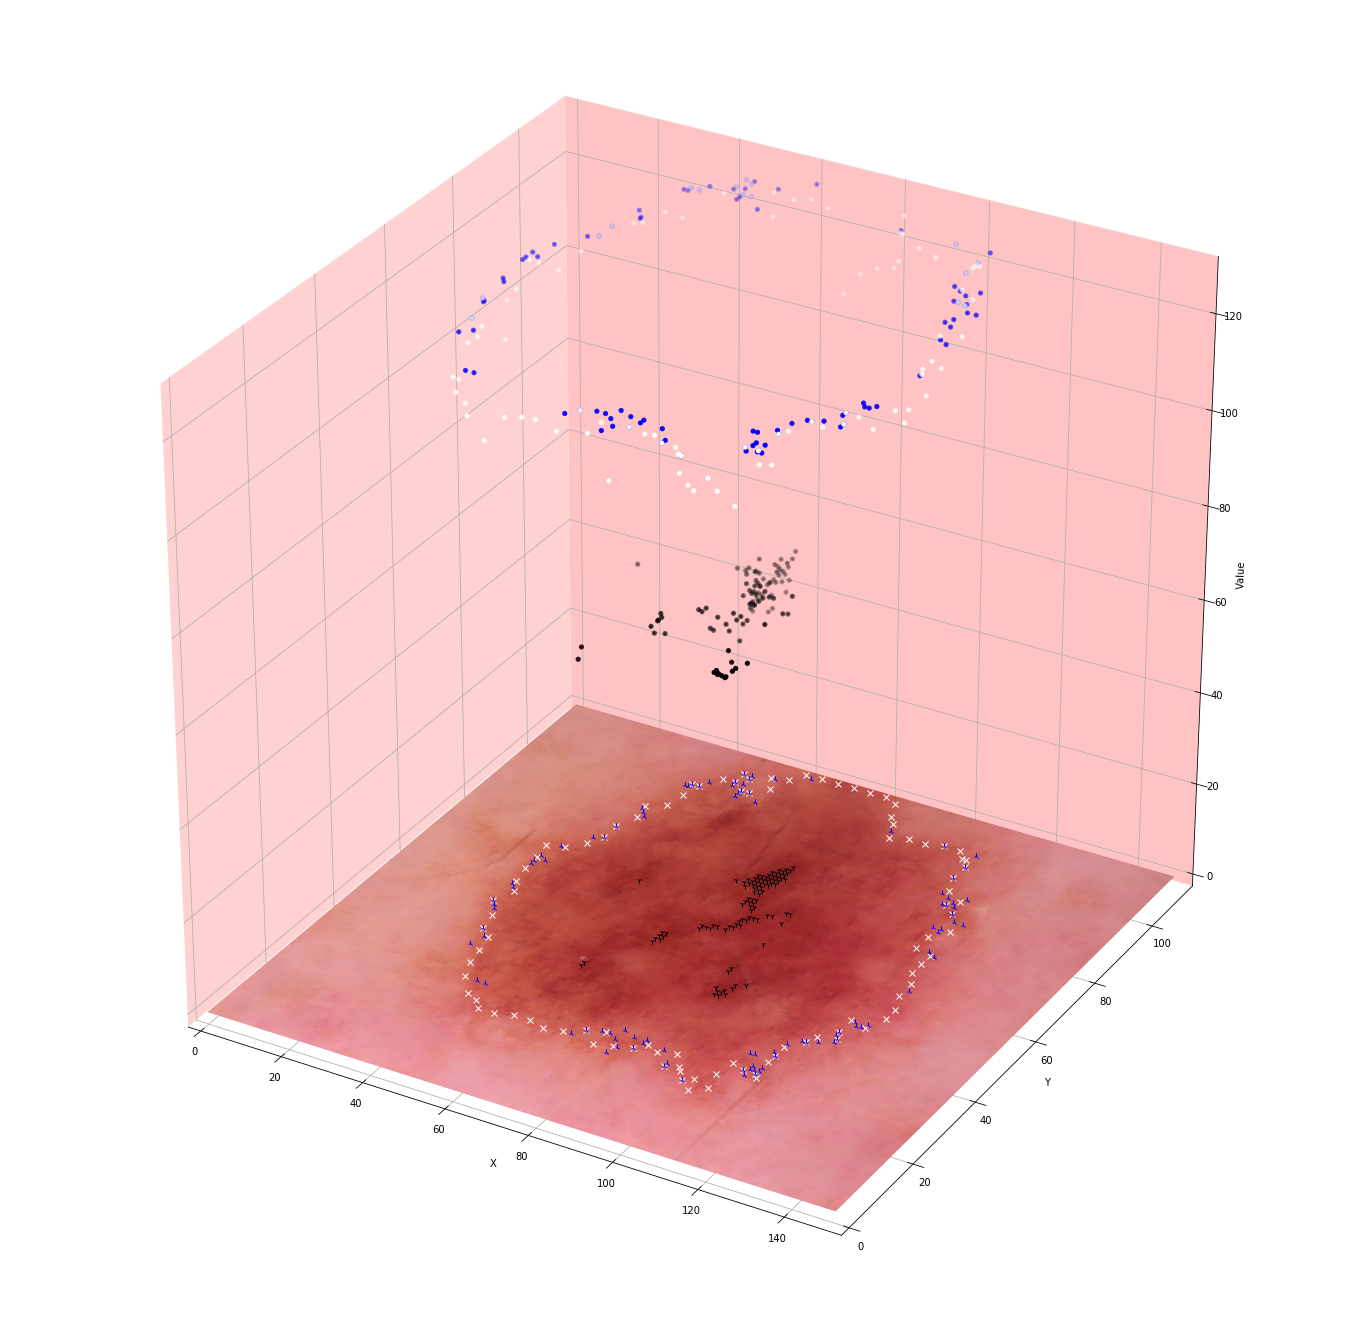
\includegraphics[width=0.8\linewidth]{TDA-figures/simple_nv20.png}
  \caption{Grayscale Simple Sampling Method}
\end{minipage}\hspace{10mm} %
\begin{minipage}{.45\textwidth}
  \centering
  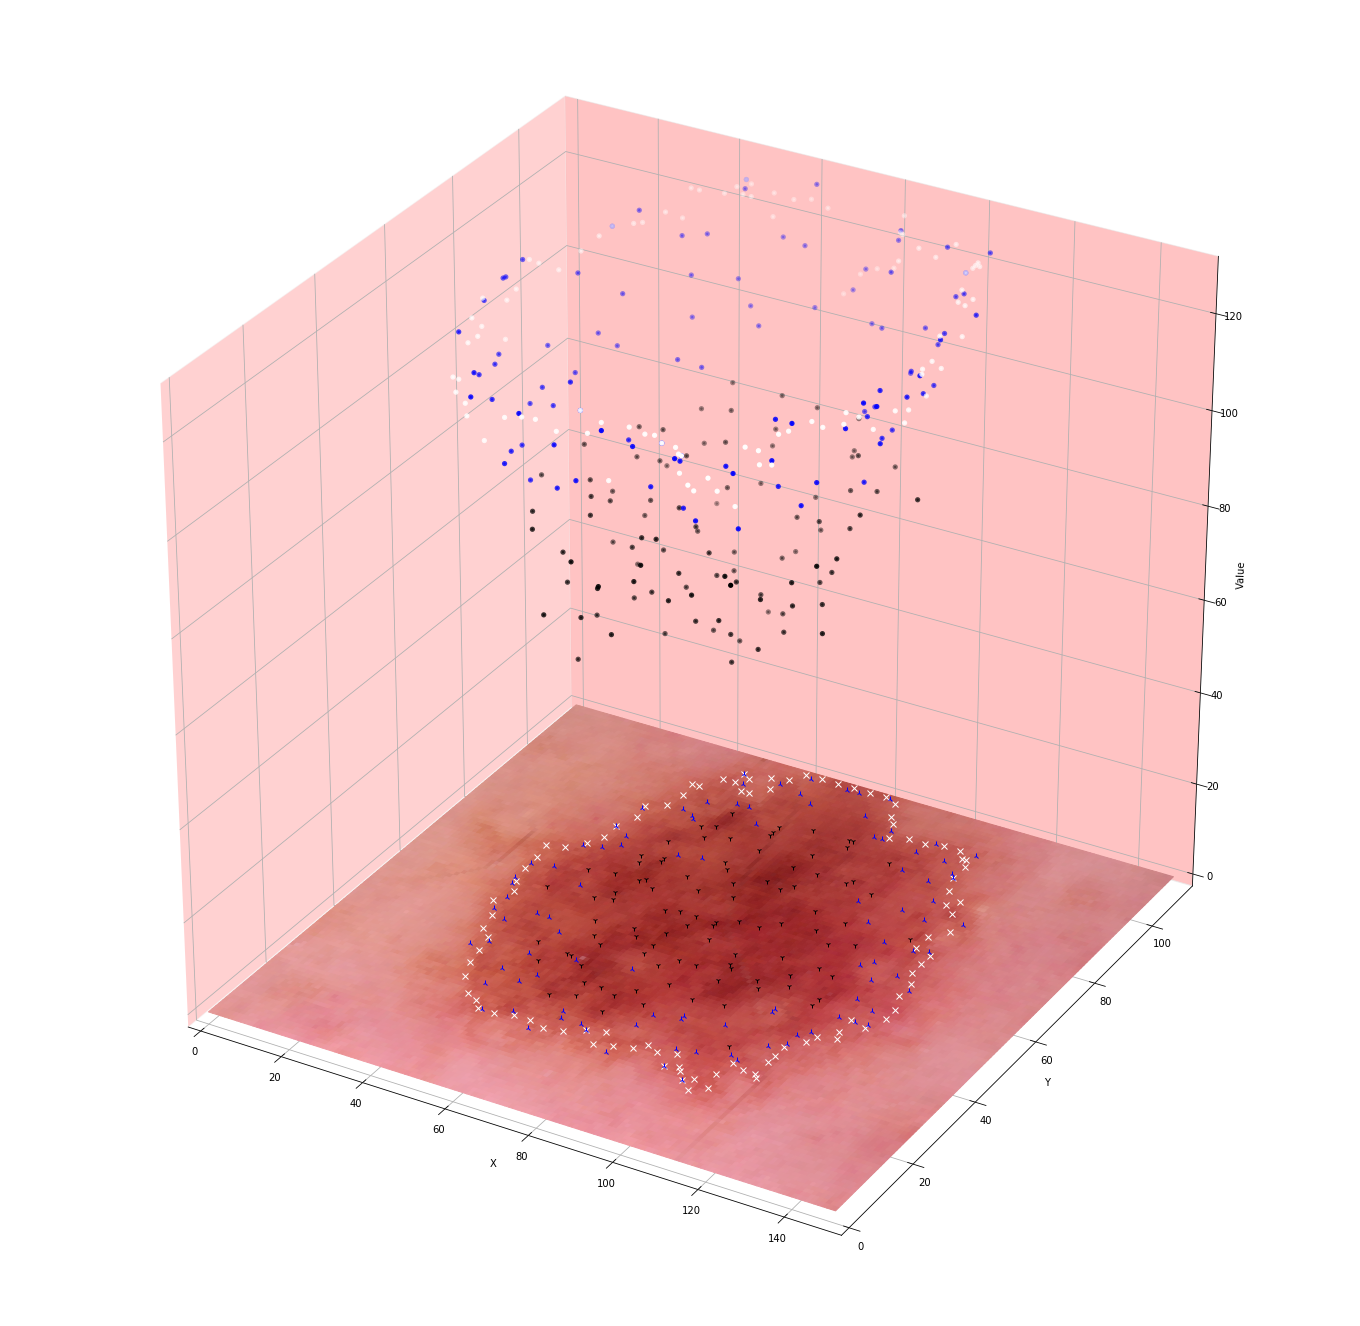
\includegraphics[width=0.8\linewidth]{TDA-figures/cluster_nv20.png}
  \caption{Grayscale Cluster Sampling Method}
\end{minipage}
\end{figure}

\centering
{\bfseries \textcolor{UF_dark_blue}{NV Image:}} Boundary (white), 100 lightest (blue), and 100 darkest (black) pixels
\end{frame}


\begin{frame}
\frametitle{Sampling Points from Skin Cancer Images}
\vspace*{-10mm}

\begin{figure}[H]
\centering
\begin{minipage}{.45\textwidth}
  \centering
  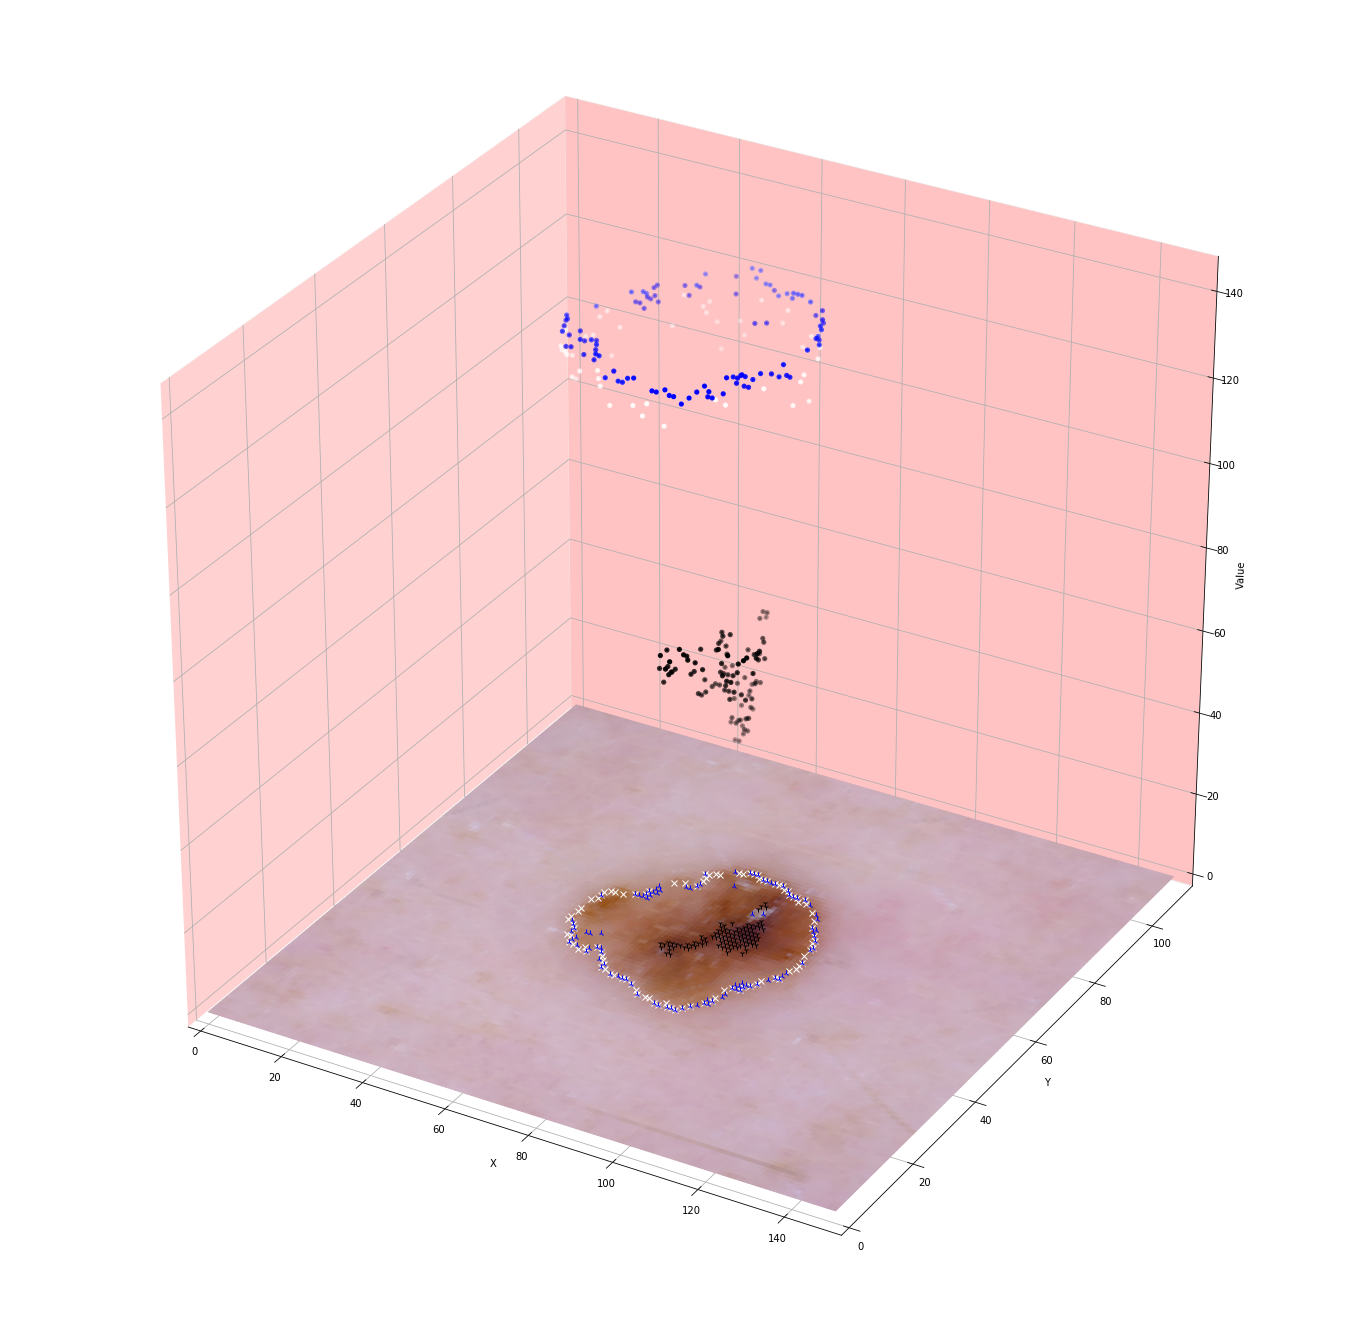
\includegraphics[width=0.8\linewidth]{TDA-figures/simple_mel4.png}
  \caption{Grayscale Simple Sampling Method}
\end{minipage}\hspace{10mm} %
\begin{minipage}{.45\textwidth}
  \centering
  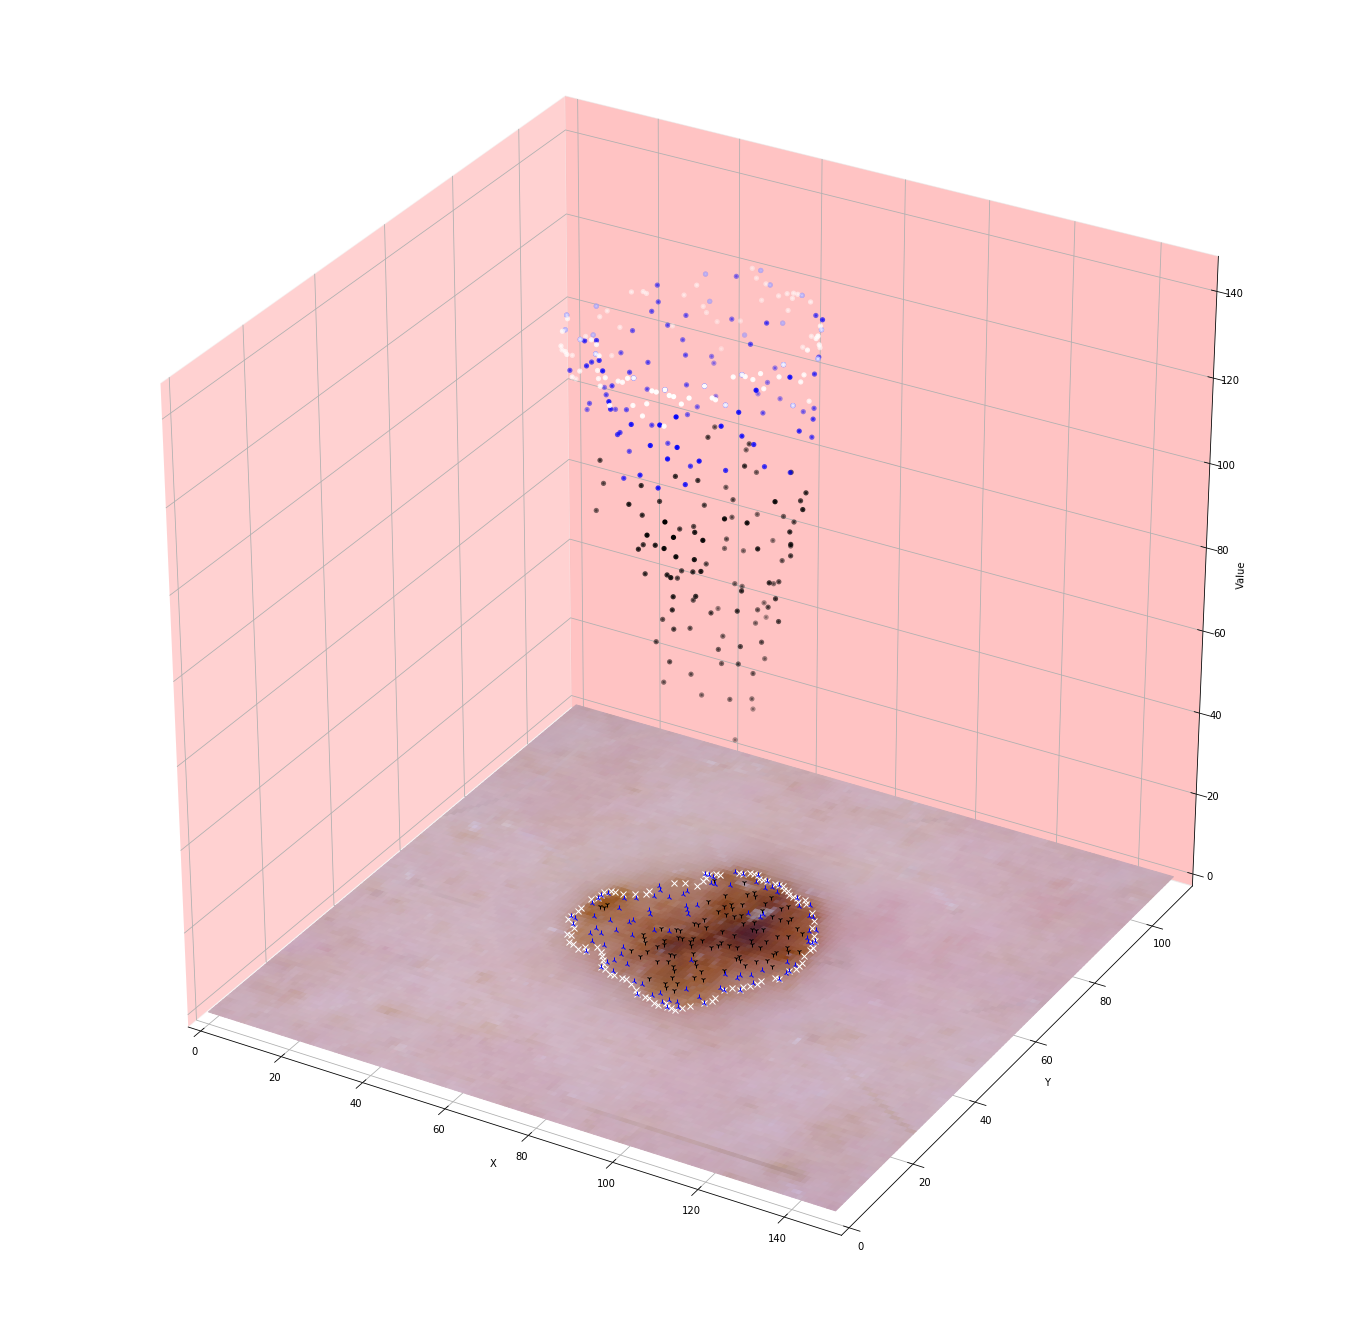
\includegraphics[width=0.8\linewidth]{TDA-figures/cluster_mel4.png}
  \caption{Grayscale Cluster Sampling Method}
\end{minipage}
\end{figure}

\centering
{\bfseries \textcolor{UF_dark_blue}{MEL Image:}} Boundary (white), 100 lightest (blue), and 100 darkest (black) pixels
\end{frame}


\iffalse
\begin{frame}
\frametitle{Sampling Points from Skin Cancer Images} \framesubtitle{Simple Method}
\begin{figure}[H]
  \centering
  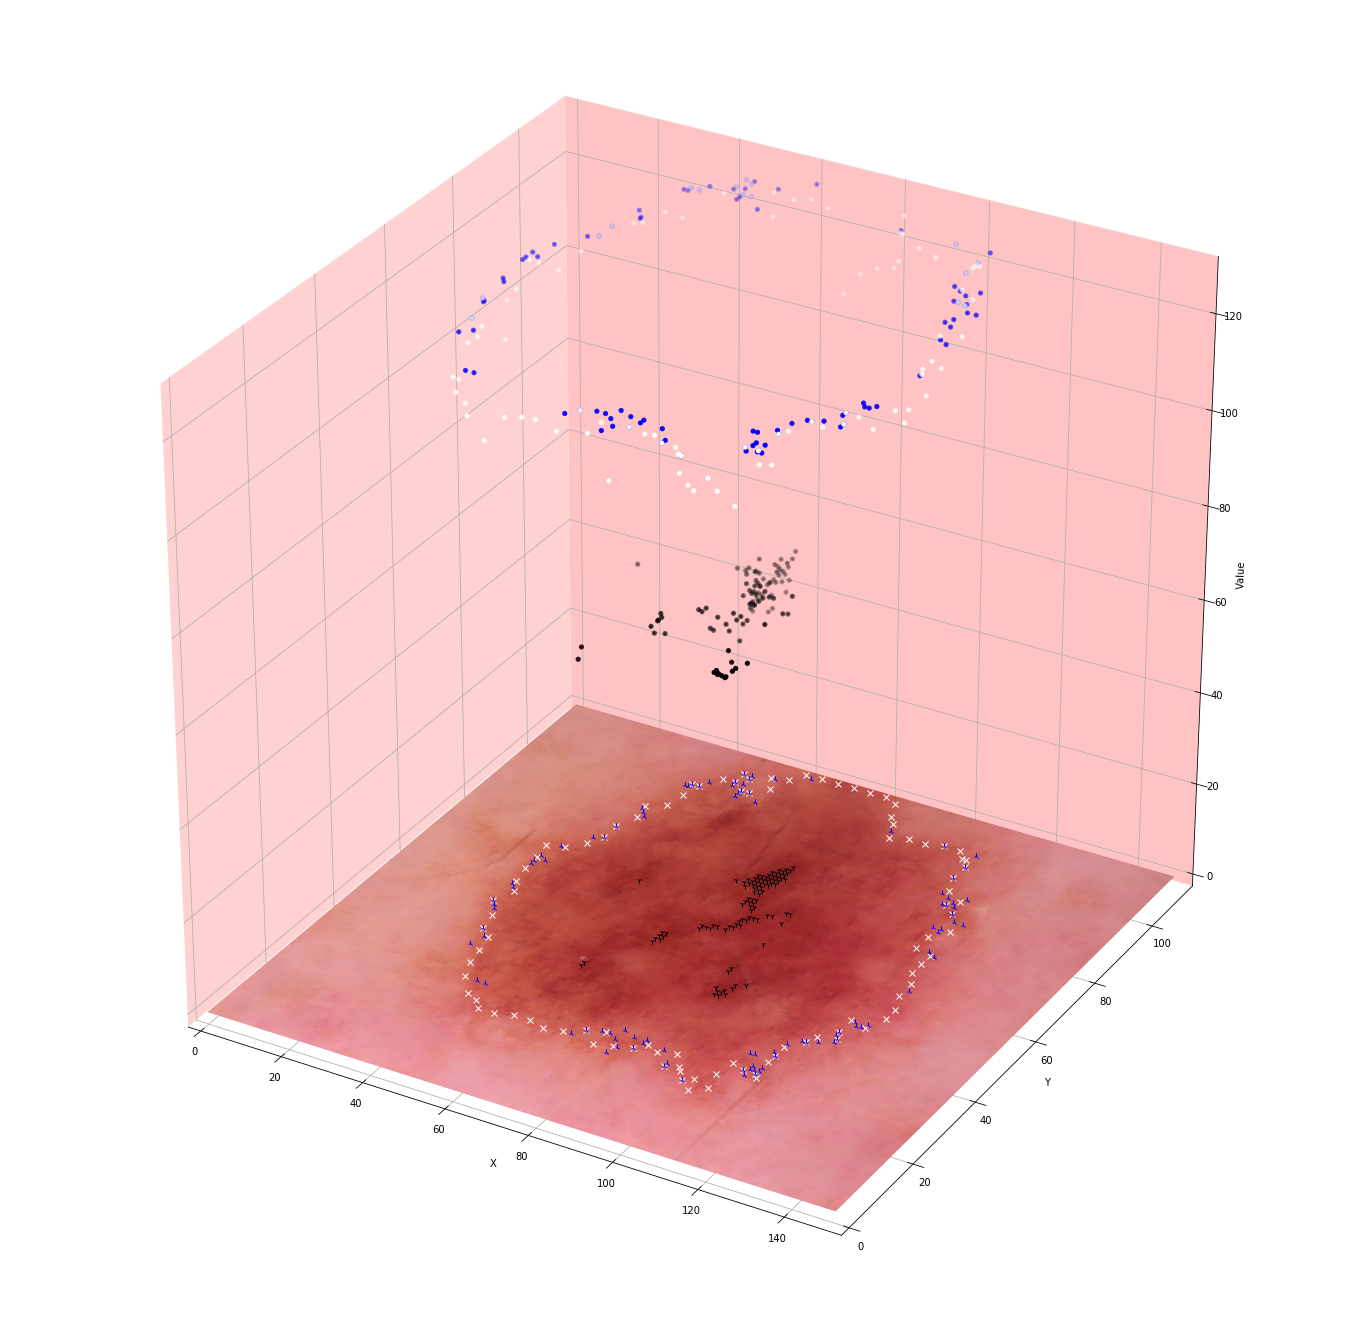
\includegraphics[width=0.4\textwidth]{TDA-figures/simple_nv20.png}
  \caption{NV Image: Boundary (white), 100 lightest (blue), and 100 darkest (black) pixels}
\end{figure}
\end{frame}

\begin{frame}
\frametitle{Sampling Points from Skin Cancer Images} \framesubtitle{Cluster Method}
\begin{figure}[H]
\centering
  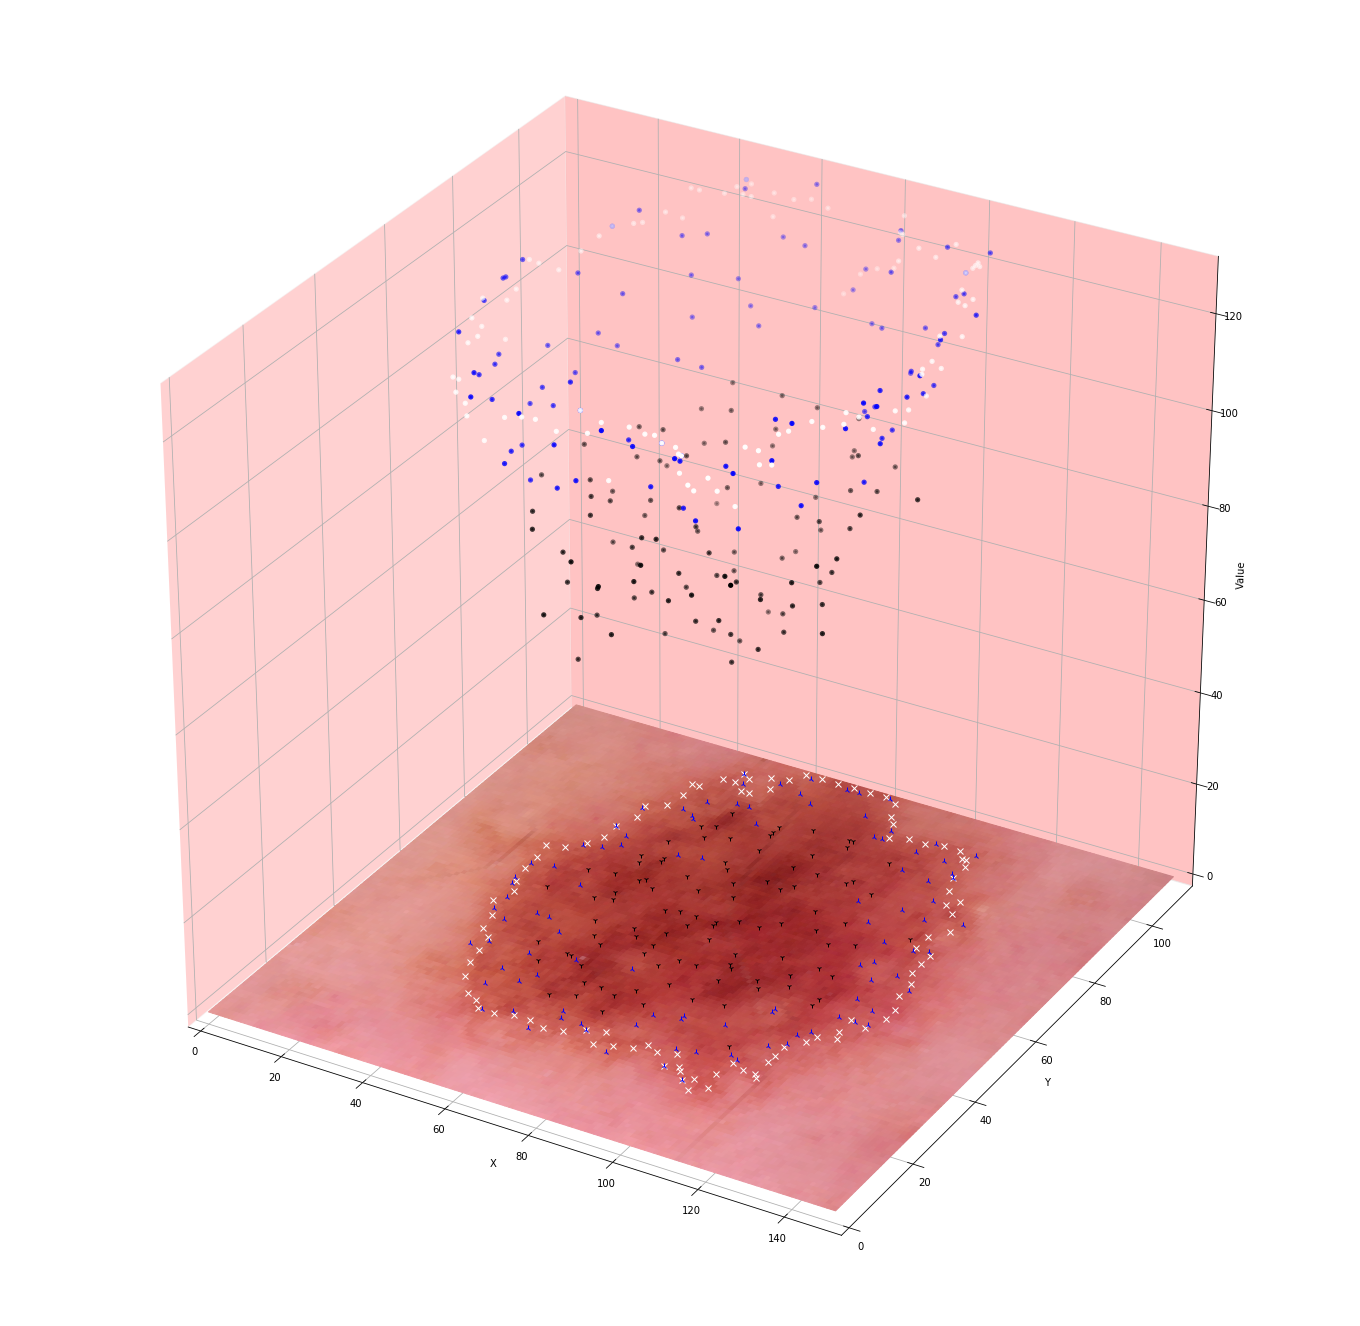
\includegraphics[width=0.4\textwidth]{TDA-figures/cluster_nv20.png}
  \caption{NV Image: Boundary (white), 100 lightest (blue), and 100 darkest (black) pixels}
\end{figure}
\end{frame}

\begin{frame}
\frametitle{Sampling Points from Skin Cancer Images} %\framesubtitle{Established Work}
\begin{figure}[H]
  \centering
  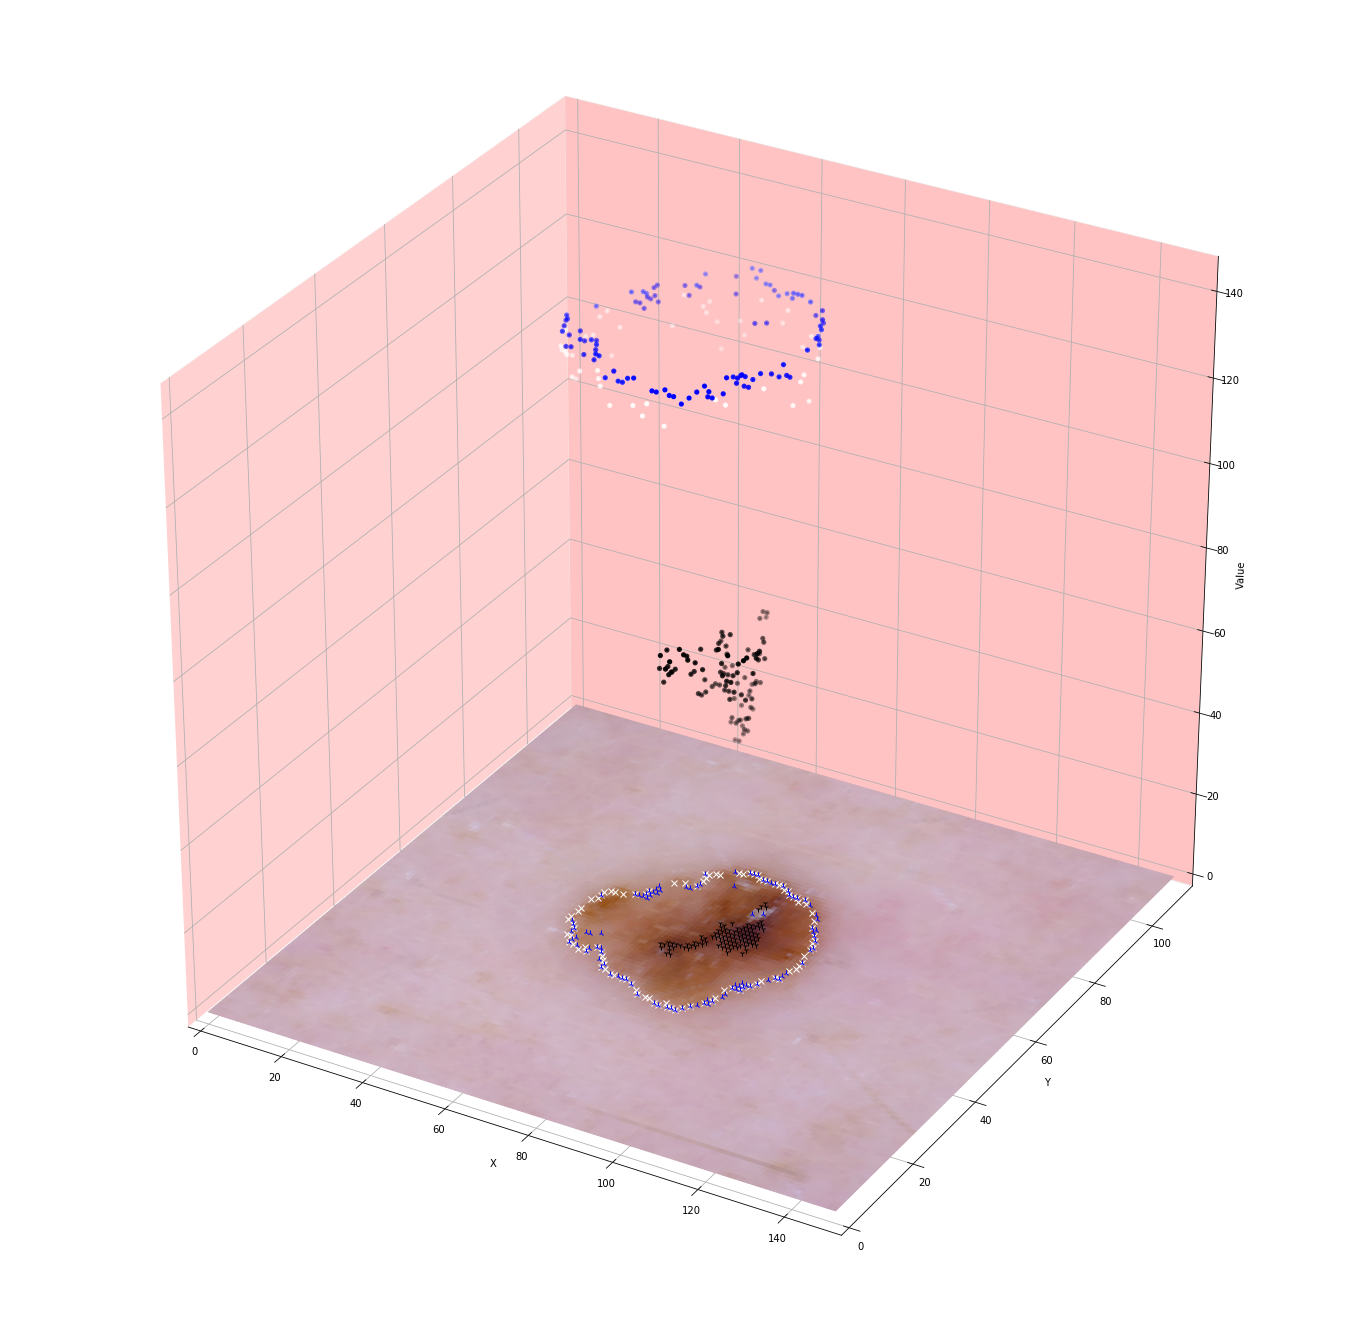
\includegraphics[width=0.4\textwidth]{TDA-figures/simple_mel4.png}
  \caption{MEL Image: Boundary (white), 100 lightest (blue), and 100 darkest (black) pixels}
\end{figure}
\end{frame}

\begin{frame}
\frametitle{Sampling Points from Skin Cancer Images} %\framesubtitle{Established Work}
\begin{figure}[H]
\centering
  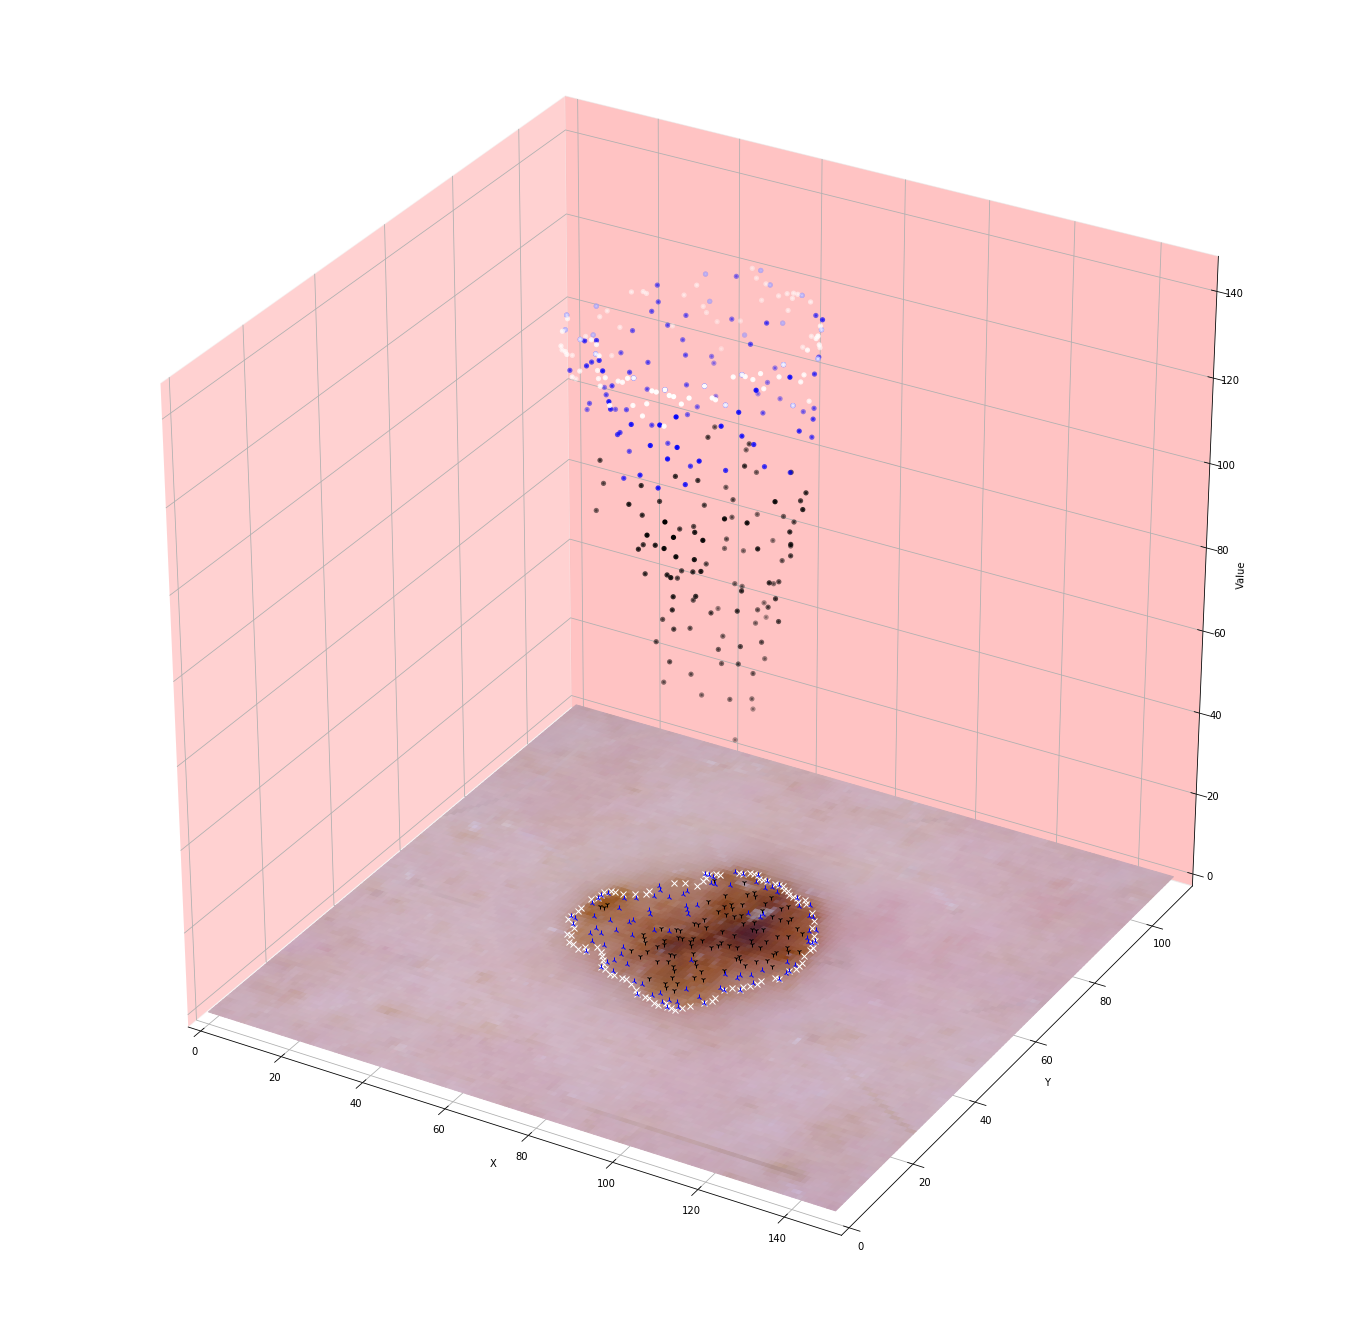
\includegraphics[width=0.4\textwidth]{TDA-figures/cluster_mel4.png}
  \caption{MEL Image: Boundary (white), 100 lightest (blue), and 100 darkest (black) pixels}
\end{figure}
\end{frame}
\fi

% ----------------------------------- TDA ----------------------------------- %
\begin{frame}
\frametitle{Computing Death Vectors and Persistence Landscapes} %\framesubtitle{Current Work}
\vspace*{-4mm}
\begin{itemize}\justifying
\item Computed persistence landscapes and death vectors with {\bfseries \textcolor{UF_dark_blue}{RStudio TDA package}}
	\begin{itemize}\justifying
	\item For each image, we used the sampled 100 boundary points and 100 darkest points from the {\bfseries \textcolor{UF_dark_blue}{simple sampling method}} for a total of {\bfseries \textcolor{UF_dark_blue}{200 points per image}}
	\item Used {\bfseries \textcolor{UF_dark_blue}{Vietoris-Rips complex}} in TDA pipeline
	\end{itemize}
\item After processing the sampled data in R, for each image we had:
	\begin{itemize}
	\item One death vector of length 199
	\item One persistence landscape vector of length 30100
	\end{itemize}
\end{itemize}
\end{frame}


\begin{frame}
\frametitle{Principal Component Analysis} \framesubtitle{Death Vectors}

\begin{figure}[H]
\centering
\begin{minipage}{.45\textwidth}
  \centering
  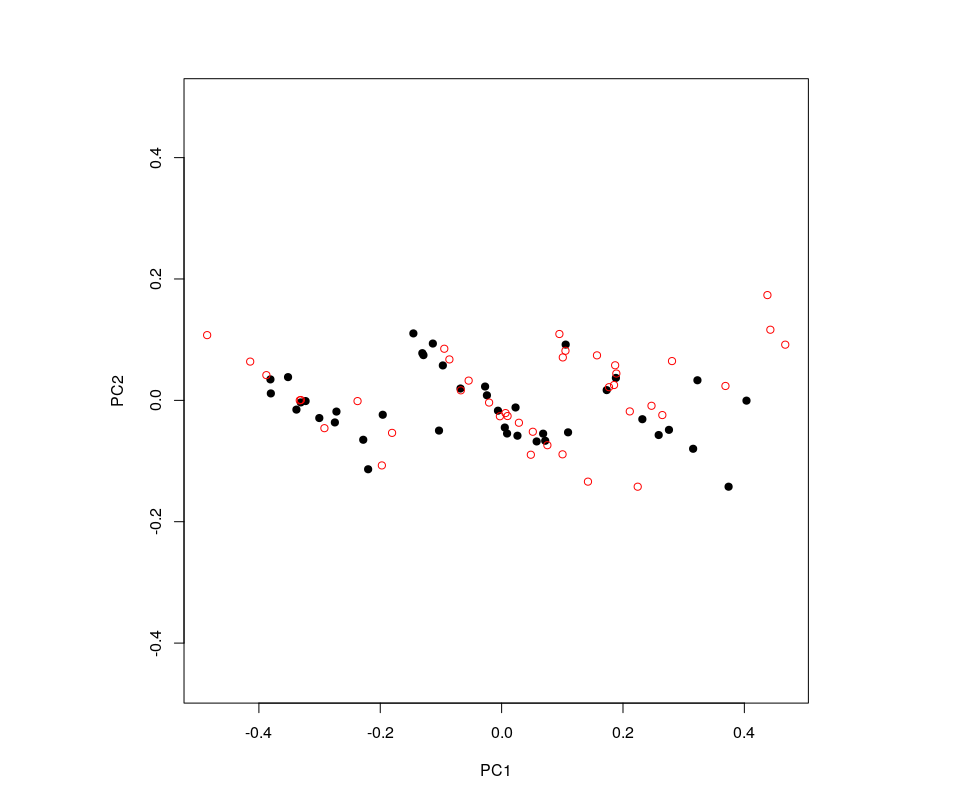
\includegraphics[width=0.8\linewidth]{TDA-figures/nv_mel_DV_PCA_Points_Plot.png}
  \caption{{\bfseries \textcolor{UF_dark_blue}{Figure 1:}} Projection of Death Vectors onto two leading PCA basis vectors}
\end{minipage}\hspace{10mm} %
\begin{minipage}{.45\textwidth}
  \centering
  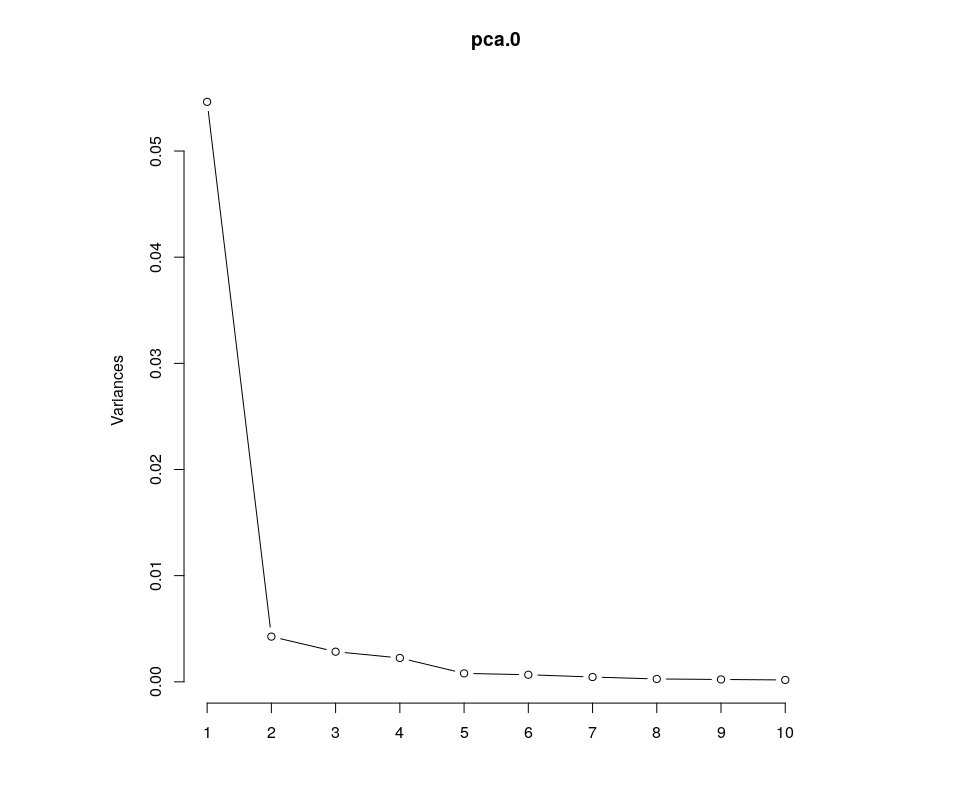
\includegraphics[width=0.8\linewidth]{TDA-figures/nv_mel_DV_PCA_Vietoris_Rips.png}
  \caption{{\bfseries \textcolor{UF_dark_blue}{Figure 2:}} Variance in direction of first ten basis vectors from PCA}
\end{minipage}
\end{figure}

\end{frame}


\begin{frame}
\frametitle{Principal Component Analysis} \framesubtitle{Pers. Landscapes}

\begin{figure}[H]
\centering
\begin{minipage}{.45\textwidth}
  \centering
  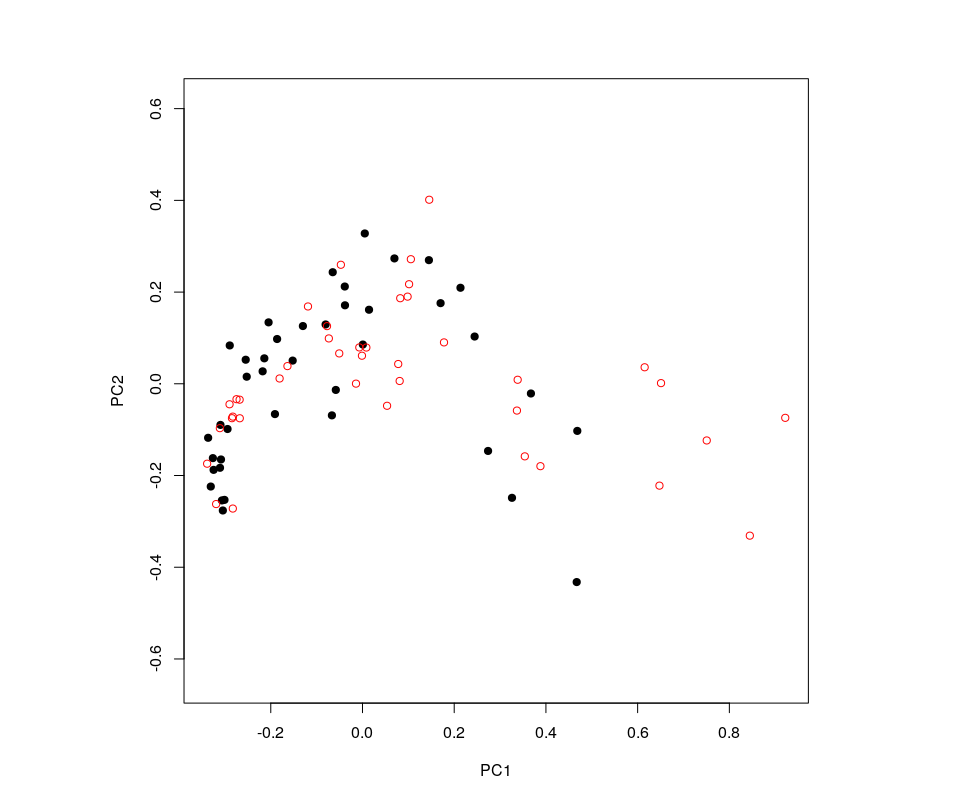
\includegraphics[width=0.8\linewidth]{TDA-figures/nv_mel_PL_PCA_Points_Plot.png}
  \caption{{\bfseries \textcolor{UF_dark_blue}{Figure 1:}} Projection of Pers. Landscapes onto two leading PCA basis vectors}
\end{minipage}\hspace{10mm} %
\begin{minipage}{.45\textwidth}
  \centering
  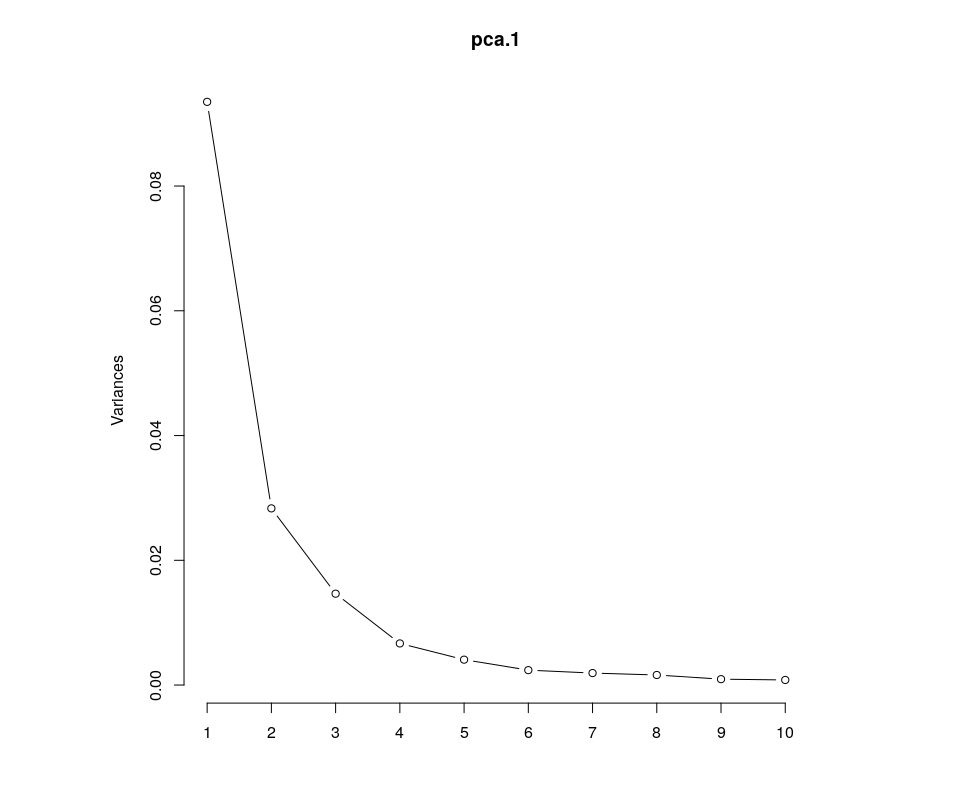
\includegraphics[width=0.8\linewidth]{TDA-figures/nv_mel_PL_PCA_Vietoris_Rips.png}
  \caption{{\bfseries \textcolor{UF_dark_blue}{Figure 2:}} Variance in direction of first ten basis vectors from PCA}
\end{minipage}
\end{figure}

\end{frame}


\begin{frame}
\frametitle{Support Vector Machine Classification} %\framesubtitle{Pers. Landscapes}

\vspace*{-6mm}
\begin{figure}[H]
\centering
  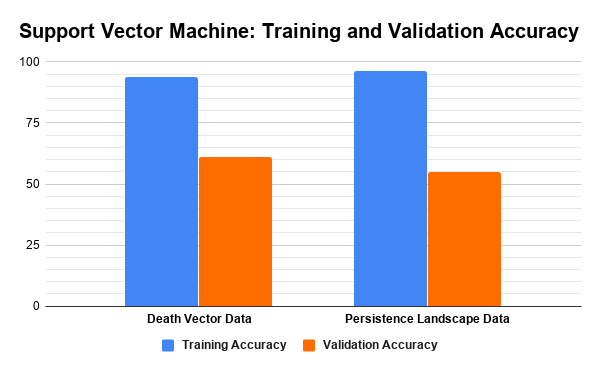
\includegraphics[width=0.55\textwidth]{TDA-figures/SVM-Graph.png}
\end{figure}

\vspace*{-2mm}
\begin{itemize}\justifying
\item Used {\bfseries \textcolor{UF_dark_blue}{R package ksvm}} with {\bfseries \textcolor{UF_dark_blue}{Gaussian radial basis function kernel}} 
	\begin{itemize}\justifying
	\item Data does not appear to be lineary separable based on the principal component analysis
	\end{itemize}
\end{itemize}

\end{frame}


\begin{frame}
\frametitle{Deep Neural Network (DNN) Classification} %\framesubtitle{Pers. Landscapes}

\begin{itemize}\justifying
\item Used Python packages {\bfseries \textcolor{UF_dark_blue}{TensorFlow}} and {\bfseries \textcolor{UF_dark_blue}{Keras}} to model and train DNNs

\item Used {\bfseries \textcolor{UF_dark_blue}{Google Colab}} with {\bfseries \textcolor{UF_dark_blue}{GPU accelerator}} to reduce training time of DNNs

\item {\bfseries \textcolor{UF_dark_blue}{Death Vector DNN}}: 
	\begin{itemize}\justifying
	\item 2 hidden layers, ReLU activation, batch normalization, dropout layers
	\item Total of {\bfseries \textcolor{UF_dark_blue}{167,506 trainable parameters}}
	\item Trained for {\bfseries \textcolor{UF_dark_blue}{120 epochs}} using {\bfseries \textcolor{UF_dark_blue}{Adam optimizer}} with {\bfseries \textcolor{UF_dark_blue}{batch size of 5}}
	\end{itemize}

\item {\bfseries \textcolor{UF_dark_blue}{Persistence Landscape DNN}}: 	
	\begin{itemize}\justifying
	\item 1 hidden layer, ReLU activation, batch normalization, dropout layers
	\item Total of {\bfseries \textcolor{UF_dark_blue}{3,015,503 trainable parameters}}
	\item Trained for {\bfseries \textcolor{UF_dark_blue}{150 epochs}} using {\bfseries \textcolor{UF_dark_blue}{Adam optimizer}} with {\bfseries \textcolor{UF_dark_blue}{batch size of 8}}
	\end{itemize}	

\end{itemize}

\end{frame}

\begin{frame}
\frametitle{Deep Neural Network (DNN) Classification} %\framesubtitle{Pers. Landscapes}

\vspace*{-6mm}
\begin{figure}[H]
\centering
  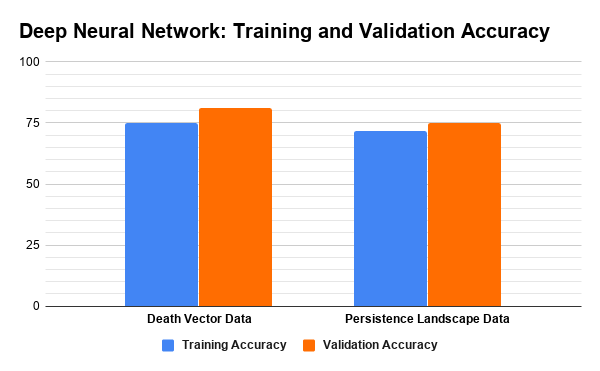
\includegraphics[width=0.75\textwidth]{TDA-figures/DNN-Graph.png}
\end{figure}

\end{frame}

% ----------------------------------- Conclusion ----------------------------------- %
\begin{frame}
\frametitle{Conclusion and Future Work} %\framesubtitle{Current Work}
\vspace*{-4mm}
\begin{itemize}\justifying
\item {\bfseries \textcolor{UF_dark_blue}{Successfully modeled and trained classifier for MEL and NV images}} that does not suffer from overfitting
\item Future work includes:
	\begin{itemize}\justifying
	\item {\bfseries \textcolor{UF_dark_blue}{Update sampling method}} to capture slightly more of internal skin cancer structure
	%\item {\bfseries \textcolor{UF_dark_blue}{Update sampling method}} to better capture density of internal skin cancer structure by using {\bfseries \textcolor{UF_dark_blue}{sklearn.cluster.DBSCAN}} or {\bfseries \textcolor{UF_dark_blue}{sklearn.cluster.AgglomerativeClustering}} and stratified sampling
	\item {\bfseries \textcolor{UF_dark_blue}{Streamline pipeline}} so sampling, TDA, and DNN classification can be done in Python
	\item {\bfseries \textcolor{UF_dark_blue}{Sample points from more images and more classes}} in HAM10000 data set
	\item Model and train DNN for {\bfseries \textcolor{UF_dark_blue}{multiclass classification}}
	\end{itemize}
\end{itemize}
\end{frame}


% ----------------------------------- Acknowledgements ----------------------------------- %
\begin{frame}
  \begin{textblock}{16}(0,6.5)
    \centering
    {\LARGE \color{white}\bf Thank you for your attention. Any questions?}
  \end{textblock}
\end{frame}
\end{document}






%
\iffalse
\begin{frame}
\frametitle{ZFP Compression Algorithm} %\framesubtitle{Established Work}
\vspace*{-3mm}
\begin{itemize} \justifying
\item[\it Step 1:]The $d$-dimensional array is partitioned into arrays of dimension $4^d$, called \emph{blocks}. The boundary is padded by zeros until an exact partition is possible.
\begin{figure}
    \centering
        \includegraphics[width=.45\textwidth]{zfp-figures/step1.pdf}
    \caption{Deconstruction of a 2-dimensional array into independent $4\times4$ blocks. If the data is not divisible by 4 the data at the boundaries is padded (shown in orange).}
    \label{fig:cut4dblock}
\end{figure}
\end{itemize}
\end{frame}
\fi
%

\begin{frame}
\frametitle{ZFP Compression Algorithm} %\framesubtitle{Established Work}
\begin{tabular}{lc}
\begin{tabular}{l}
\parbox{0.4\linewidth}{
\begin{itemize} \justifying
\item[\it Step 2:] For each block, convert \\ \vspace{3mm}
\begin{center}
{\bfseries Floating-point} \vspace{2mm} \\ %in each block 
$\bm{\Downarrow}$ \vspace{2mm} \\
{\bfseries Block-floating-point} \vspace{3mm} \\
\end{center}
using a common exponent for each block \cite{MitrablockRoundingError} and integers in two's complement format. %where we write $q$ to denote the number of bits used in two's complement. %The block-floating point representation is then shifted and rounded to $4^d$ signed integers as seen in Figure \ref{fig:bfprepresentation}.
\end{itemize}
}
\end{tabular}
\hspace{-9mm} & \begin{tabular}{c}
    \includegraphics[width=0.7\linewidth]{zfp-figures/step3.pdf}
\end{tabular}
\end{tabular}

\rule{5cm}{0.5pt}
\parbox{\textwidth}{\fontsize{6}{8}\selectfont
\begin{itemize}
\item[\cite{MitrablockRoundingError}] Abhijit Mitra, \textit{On Finite Wordlength Properties of Block-Floating-Point Arithmetic}, International Journal of Electrical, Computer, Energetic, Electronic and Communication Engineering, 2008
\end{itemize}
}
\end{frame}

\begin{frame}
\frametitle{ZFP Compression Algorithm} %\framesubtitle{Established Work}
\begin{tabular}{lc}
\begin{tabular}{l}
\parbox{0.54\linewidth}{
\begin{itemize} \justifying
\item[\it Step 3:] {\bfseries Decorrelate integers using custom, high-speed, near orthogonal transform} that is similar to discrete cosine transform; both of which have the \emph{energy compaction property} that concentrates information in each block to low frequency transform\\ coefficients.
\end{itemize}
}
\end{tabular}
\hspace{-9mm} & \begin{tabular}{c}
\parbox{0.46\linewidth}{
\begin{center}
$\bm{L_d = \underbrace{L \otimes L \otimes \cdots \otimes L}_{(d-1) \ \text{products}}}$ \\
\vspace{3mm}
where
\vspace*{-2.5mm}
\end{center}
\begin{align*}{\tiny
\bm{L} = \frac{1}{16} \begin{bmatrix}
4 & 4 & 4 & 4 \\
5 & 1 & -1 & -5 \\
-4 & 4 & 4 & -4 \\
-2 & 6 & -6 & 2
\end{bmatrix}
}
\end{align*}
}
\end{tabular}
\end{tabular}
\end{frame}

%
\iffalse
\begin{frame}
\frametitle{ZFP Compression Algorithm} %\framesubtitle{Established Work}
\begin{itemize} \justifying
\item[\it Step 3:] {\bfseries Integers are decorrelated using a custom, high-speed, near orthogonal\\ transform} that is similar to the discrete cosine transform; both of which have the \emph{energy compaction property} that concentrates the information within the block to low frequency transform coefficients.
\end{itemize}
\end{frame}
\fi
%

%
\iffalse
\begin{frame}
\frametitle{ZFP Compression Algorithm} %\framesubtitle{Established Work}
\vspace*{-3mm}
\begin{figure}
    \centering
        \includegraphics[width=\textheight]{figures/step3.pdf}
    \caption{Floating-point bit representation in single precision converted to a block-floating-point representation and its corresponding signed integers. %Note that, depending on the relative disparity of the 16 numbers, some truncation may occur for the numbers of the smallest magnitude.
    }
   \label{fig:bfprepresentation}
\end{figure}
\end{frame}
\fi
%

\begin{frame}
\frametitle{ZFP Compression Algorithm} %\framesubtitle{Established Work}
\begin{tabular}{lc}
\begin{tabular}{l}
\parbox{0.46\linewidth}{
\begin{itemize} \justifying
\item[\it Step 4:] {\bfseries Reorder coefficients by total\\ sequency} as transform coefficients corresponding to low frequencies tend to be larger in magnitude \cite{zfp-doc}.
\end{itemize}
}
\end{tabular}
\hspace{-9mm} & \begin{tabular}{c}
    \includegraphics[width=.62\linewidth]{zfp-figures/step4.pdf}
\end{tabular}
\end{tabular}
\rule{5cm}{0.5pt}
\parbox{\textwidth}{\fontsize{6}{8}\selectfont
\begin{itemize}
\item[\cite{zfp-doc}] Peter Lindstrom, \textit{ZFP Documentation (version 0.5.4)}, October 2018
\end{itemize}
}
\end{frame}


%
\iffalse
\begin{frame}
\frametitle{ZFP Compression Algorithm} %\framesubtitle{Established Work}
\vspace*{-3mm}
\begin{itemize} \justifying
\item[\it Step 4:] {\bfseries Reorder coefficients by total sequency} since transform coefficients corresponding to low frequencies tend to be larger in magnitude \cite{zfp-doc}.
\begin{figure}
    \centering
        \includegraphics[width=.5\textwidth]{zfp-figures/step4.pdf}
    \caption{Total sequency ordering for a 2-dimensional array, which groups the diagonal elements together. }
    \label{fig:totalsequency}
\end{figure}
\end{itemize}
\end{frame}
\fi
%

%
\iffalse
\begin{frame}
\frametitle{ZFP Compression Algorithm} %\framesubtitle{Established Work}
\begin{itemize} \justifying
\item[\it Step 5:] For each block, convert \\ \vspace{3mm}
\begin{center}
{\bfseries Two's complement:} %signed integers 
$x = -a_{N-1} 2^{N-1}  + \sum_{i = 0}^{N-2} a_i 2^i$ \vspace{2mm} \\ %in each block 
$\bm{\Downarrow}$ \vspace{2mm} \\
{\bfseries Negabinary \cite{Knuth}: } $x = \sum_{i = 0}^{N-1} d_i (-2)^i$ \vspace{3mm} \\
\end{center}
where each $a_i, d_i \in \{ 0, 1 \}$.
%\item[\it Step 6:] The bits that represent the list of $4^d$ integers are transposed so that they are ordered by bit plane, from most to least significant bit, instead of by coefficient.  
\item[\it Step 7:] Compress each bit plane losslessly using {\bfseries embedded coding}, which exploits the property that the transform coefficients tend to have many leading zeros. %As this step is lossless, the encoding details are omitted.  
\end{itemize}
\end{frame}
\fi
%


\begin{frame}
\frametitle{ZFP Compression Algorithm} %\framesubtitle{Established Work}
\begin{itemize} \justifying
\item[\it Step 5:] {\bfseries Two's complement} signed integers $\Longrightarrow$ {\bfseries negabinary} integers~\cite{Knuth} %ensures that the error caused by the remaining steps is centered around zero.
\begin{align*}
{\textbf{ Negabinary: }} x = \sum_{i = 0}^{N} d_i (-2)^i,
\end{align*}
where each $d_i \in \{ 0, 1 \}$.
%\item[\it Step 6:] The bits that represent the list of $4^d$ integers are transposed so that they are ordered by bit plane, from most to least significant bit, instead of by coefficient.  
\item[\it Step 7:] Compress each bit plane losslessly using {\bfseries embedded coding}, which exploits the property that the transform coefficients tend to have many leading zeros. %As this step is lossless, the encoding details are omitted.  
\end{itemize}

\rule{5cm}{0.5pt}
\parbox{\textwidth}{\fontsize{6}{8}\selectfont
\begin{itemize}
\item[\cite{Knuth}] Donald Knuth, \textit{The Art of Computer Programming, Volume 2 (3rd Ed.): Seminumerical Algorithms}, Addison-Wesley Longman Publishing Co., Inc., 1997
\end{itemize}
}
\end{frame}


\begin{frame}
\frametitle{ZFP Compression Algorithm} %\framesubtitle{Established Work}
\begin{tabular}{lc}
\begin{tabular}{l}
\parbox{0.46\linewidth}{
\begin{itemize} \justifying
\item[\it Step 8:] Embedded coder {\bfseries emits one bit at a time until stopping criteria are satisfied} for specified mode: %. The exact stopping criteria is dependent on the mode of ZFP compression: either
	\begin{itemize}
	\item Fixed precision
	\item Fixed rate
	\item Fixed accuracy
	\end{itemize} 
\end{itemize}
}
\end{tabular}
\hspace{-5mm} & \begin{tabular}{c}
    \includegraphics[width=.54\linewidth]{zfp-figures/bit-plane.pdf}
\end{tabular}
\end{tabular}
\end{frame}


\begin{frame}
\frametitle{ZFP Compression Algorithm} %\framesubtitle{Established Work}
\begin{tabular}{lc}
\begin{tabular}{l}
\parbox{0.46\linewidth}{
\begin{itemize} \justifying
\item[\it Step 8:] Embedded coder {\bfseries emits one bit at a time until stopping criteria are satisfied} for specified mode: %. The exact stopping criteria is dependent on the mode of ZFP compression: either
	\begin{itemize}
	\item {\bfseries Fixed precision}
	\item \textcolor{black!50}{Fixed rate}
	\item \textcolor{black!50}{Fixed accuracy}
	\end{itemize} 
\end{itemize}
}
\end{tabular}
\hspace{-5mm} & \begin{tabular}{c}
    \includegraphics[width=.54\linewidth]{zfp-figures/bit-plane-trunc.pdf}
\end{tabular}
\end{tabular}
\end{frame}


%
\iffalse
\begin{frame}
\frametitle{ZFP Compression Algorithm} %\framesubtitle{Established Work}
\begin{itemize} \justifying
\item[\it Step 8:] Embedded coder emits one bit at a time until stopping criteria are satisfied for specified mode: %. The exact stopping criteria is dependent on the mode of ZFP compression: either
{\bfseries Fixed precision}, fixed rate, or fixed accuracy.   
\end{itemize}
\begin{figure}
    \vspace*{-3mm}
    \centering
        \includegraphics[width=.60\textwidth]{figures/bit-plane.pdf}
%    \caption{Step 8 of ZFP Compression.}
    \label{fig:step8.1}
\end{figure}
\end{frame}

\begin{frame}
\frametitle{ZFP Compression Algorithm} %\framesubtitle{Established Work}
\begin{itemize} \justifying
\item[\it Step 8:] Embedded coder emits one bit at a time until stopping criteria are satisfied for specified mode: %. The exact stopping criteria is dependent on the mode of ZFP compression: either
{\bfseries Fixed precision}, fixed rate, or fixed accuracy.  
\end{itemize}
\begin{figure}
    \vspace*{-3mm}
    \centering
        \includegraphics[width=.60\textwidth]{figures/bit-plane-trunc.pdf}
%    \caption{Step 8 of ZFP Compression.}
    \label{fig:step8.2}
\end{figure}
\end{frame}
\fi
%


% ----------------------------------- ZFP Error Analysis ----------------------------------- %
\begin{frame}
\frametitle{ZFP Error Analysis - Definitions}
\justifying
\vspace{-3mm}
Let $\mathbb{B} = \{ 0, 1 \}$ and define $\mathcal{C} := \left\{ \{ c_i \}_{i = -\infty}^{\infty} : c_i \in \mathbb{B} \ \text{for all} \ i \in \mathbb{Z} \right\}$. %For $c \in \mathcal{C}$, we define the \textbf{active bit set of $c$} by $\mathcal{I} (c) := \{ i \in \mathbb{Z} : c_i = 1 \}$.
For $x \in \mathbb{R}$, there exist $c, d \in \mathcal{C}$ and $p \in \mathbb{B}$ such that %$x$ can be represented in signed binary and negabinary as 
\begin{align}
{\textbf{Signed Binary: }} x = (-1)^p \sum_{i = - \infty}^{\infty} c_i 2^i \ \ \ \text{ and}  \ \ \ {\textbf{ Negabinary: }} x = \sum_{i = - \infty}^{\infty} d_i (-2)^i. \label{CrepX}
\end{align}
As such, there exist $\mathcal{A}, \mathcal{N} \subset \mathcal{C}$ such that, for each $x \in \mathbb{R}$, there exist unique
elements $c \in \mathcal{A}$, $p \in \mathbb{B}$, and $d \in
\mathcal{N}$ such that $x$ can be represented in the binary and
negabinary form in (\ref{CrepX}) using $c$, $p$, and $d$,
respectively. %In particular, we choose $\mathcal{A}$ and $\mathcal{N}$ such that $\mathcal{I} (c)$ and $\mathcal{I} (d)$ are finite whenever possible. This choice is made so that elements can be represented using finitely many nonzero bits.
\vspace{4mm}

For simplicity define $\mathcal{B} := \{ (p, a) \in  \mathbb{B} \times \mathcal{A} : (p, a) \neq ( 1, 0_{\mathcal{C}} ) \}$.
\end{frame}


% ----------------------------------- ZFP Error Analysis ----------------------------------- %
\begin{frame}
\frametitle{ZFP Error Analysis - Definitions}
\justifying
\vspace*{-3mm}
We now define $f_\cB : \mathcal{B} \to \mathbb{R}$ and $f_\cN : \mathcal{N} \to \mathbb{R}$ by 
\begin{align*}
f_\cB (b) &= (-1)^{{p}} \sum_{i = -\infty}^{\infty} a_i 2^i, \ \ \ \ \ \text{for all} \ b = ({p}, a) \in \mathcal{B}, \\
f_\cN (d) &= \sum_{i = -\infty}^{\infty} d_i (-2)^i, \ \ \ \ \ \text{for all} \ d \in \mathcal{N}.
\end{align*}
By our choice of $\mathcal{B}$ and $\mathcal{N}$, $f_\cB$ and $f_\cN$ are bijections and with inverses denoted by $f_\cB^{-1} : \mathbb{R} \to \mathcal{B}$ and $f_\cN^{-1} : \mathbb{R} \to \mathcal{N}$, respectively.
\vspace{6mm}

Using these maps, {\bfseries we can define binary operations under which $\cB$ and $\cN$ are fields}. Then we can work with vector spaces over $\cB$ and $\cN$.
\end{frame}


% ----------------------------------- ZFP Error Analysis ----------------------------------- %
\begin{frame}
\frametitle{ZFP Error Analysis - Definitions}
\vspace*{-3mm}
\justifying
%We now wish to determine norms $\| \cdot \|_{\mathcal{B}, p} : \mathcal{B}^n \to [0, \infty)$ under which $F_{\mathcal{B}} : \mathcal{B}^n \to \mathbb{R}^n$ is an isometry
We obtain normed vector spaces by defining $\| \cdot \|_{\mathcal{B}, p} : \mathcal{B}^n \to [0, \infty)$ by 
\begin{align*}
	\| \bm{a} \|_{\mathcal{B}, p} = \left\{ \begin{array}{ccc} 
	\displaystyle \left( \sum_{i = 1}^{n} \left| f_\cB(\bm{a}_i) \right|^{p} \right)^{1/p} &: & 1 \leq p < \infty \\
	\displaystyle \max_{1 \leq i \leq n} \left| f_\cB(\bm{a}_i) \right| &: & p = \infty \\
	\end{array} \right. %\label{BpNorm}
\end{align*}
%The following result is an immediate consequence from the definition of $\| \cdot \|_{\mathcal{B}, p}$.
\begin{lemma}[D, Fox, Hittinger, Lindstrom, Sanders (2018)]
\label{BNormLemma}
For all $\bm{a} \in \mathcal{B}^n$, $\bm{x} \in \mathbb{R}^n$, and $1 \leq p \leq \infty$, $\| \cdot \|_{\mathcal{B}, p}$ is a norm satisfying 
\begin{align*}
\| F_\cB (\bm{a}) \|_p = \| \bm{a} \|_{\mathcal{B}, p} \ \ \ \text{and} \ \ \ \| \bm{x} \|_p = \| F_\cB^{-1} (\bm{x}) \|_{\mathcal{B}, p}.
\end{align*}
\end{lemma}
\end{frame}


% ----------------------------------- ZFP Error Analysis ----------------------------------- %
\begin{frame}
\frametitle{ZFP Error Analysis - Step 2}
\justifying
\vspace*{-3mm}
\begin{figure}
    \centering
        \includegraphics[width=\textheight]{zfp-figures/step3.pdf}
    \caption{Floating-point bit representation in single precision converted to a block-floating-point representation and its corresponding signed integers in Step 2 of ZFP. %Note that, depending on the relative disparity of the 16 numbers, some truncation may occur for the numbers of the smallest magnitude.
    }
   \label{fig:bfprepresentation}
\end{figure}
\end{frame}


% ----------------------------------- ZFP Error Analysis ----------------------------------- %
\begin{frame}
\frametitle{ZFP Error Analysis - Step 2}
\justifying
%To illustrate our approach, we now consider the lossy and lossless operators for one step of ZFP. 
{\bfseries Lossy} and {\bfseries lossless compression operators} for step 2 are $\tilde{C}_2, C_2:\mathbb{R}^{4^d} \rightarrow \cB^{4^d}$ where 
\begin{align*}
\tilde{C}_2 (\bm{x}) := T_{\mathcal{S}} S_{\ell} F_{\cB}^{-1}(\bm{x}) \ \ \ \ \text{and} \ \ \ \ C_2(\bx ) := S_{\ell}F_{\cB}^{-1} (\bx),
\end{align*}
%\text{ for all } \bm{x} \in \mathbb{R}^{4^d}
where $\mathcal{S} := \{
i \in \mathbb{Z} : i \geq 0 \}$, $\ell = e_{max}(F_\cB^{-1}(\bx))- q+1$, the \textbf{truncation operator},
$t_{\mathcal{S}} : \mathcal{C} \to \mathcal{C}$, is defined by  
\begin{align*}
t_{\mathcal{S}} (c)_i = \left\{ \begin{array}{ccc} 
                c_i &: & i \in \mathcal{S} \\
                0 &: & i \not\in \mathcal{S} \\
                \end{array} \right., \ \ \ \text{for all} \ c \in \mathcal{C} \ \text{and all} \ i \in \mathbb{Z},
\end{align*}
and the \textbf{shift operator}, $s_{\ell} :
\mathcal{C} \to \mathcal{C}$, is defined by 
\begin{align*}
s_{\ell} (c)_i = c_{i + \ell}, \ \ \ \text{for all} \ c \in \mathcal{C} \ \text{and all} \ i \in \mathbb{Z}.
\end{align*}
\end{frame}


% ----------------------------------- ZFP Error Analysis ----------------------------------- %
\begin{frame}
\frametitle{ZFP Error Analysis - Step 2}
\justifying
{\bfseries Lossy decompression operator} for step 2 undoes the shift in $\tilde{C}_2$ and converts each component back to a floating point representation. Hence, $\tilde{D}_2: {\cB}^{4^d}\rightarrow \mathbb{R}^{4^d}$ is given by 
\begin{align*}
	\tilde{D}_2(\ba) := F_{\cB} S_{-\ell} fl_k (\ba), \ \text{for all} \ \bm{a} \in
	\mathcal{{\cB}}^{4^d},
\end{align*}
where $fl_k (\ba)_i$ %converts each component to 
denotes a floating point resepresentation with $k$ mantissa bits. \\
\vspace{5mm} 
The {\bfseries lossless decompression operator} $D_2: {\cB}^{4^d}\rightarrow \mathbb{R}^{4^d}$ is defined as
\begin{align*}
	D_2(\ba) := F_{\cB} S_{-\ell}(\ba), \ \text{for all} \ \bm{a} \in \mathcal{{\cB}}^{4^d}.
\end{align*}
\end{frame}


%
\iffalse
% ----------------------------------- ZFP Error Analysis ----------------------------------- %
\begin{frame}
\frametitle{ZFP Error Analysis - Step 2}
\justifying
\begin{prop}[Diffenderfer, Fox, Hittinger, Lindstrom, Sanders (2018)]
Suppose $\bm{x} \in \mathbb{R}^{4^d}$ and $\bm{a} \in \cB^{4^d}$, such that $e_{max,\cB}(F_\cB (\ba)) = q-1.$
	\label{Step2Prop}
	\begin{itemize}
		\item[(i)] Then $\| \tilde{C}_2 \bx - C_2 \bx \|_{\infty} \leq 2^{-\ell} \epsilon_{q} \| \bm{x} \|_{\infty}$. 
		\item[(ii)] Then $\| \tilde{D}_2 \ba - D_2 \ba \|_{\infty} \leq 2^{\ell} \epsilon_{k} \| \bm{a} \|_{\infty}$. 
	\end{itemize}
where $\epsilon_n = 2^{1-n}$, for $n \in \mathbb{Z}$.
\end{prop}
\end{frame}
\fi
%

% ----------------------------------- ZFP Error Analysis ----------------------------------- %
\begin{frame}
\frametitle{ZFP Error Analysis} %\framesubtitle{Step 2}
\begin{itemize}\justifying
\item {\bfseries Repeat for each step of ZFP} until we have established error bounds for each set of compression and decompression operators.
\item {\bfseries Compose operators for each step} to define lossy ZFP compression/decompression operators by
\begin{align*}
		\tilde{C} (\bm{x}) = \left( \tilde{C}_{8} \circ {C}_{5} \circ {C}_{4} \circ \tilde{C}_{3} \circ \tilde{C}_{2} \right) (\bm{x}), \ \ \ \text{for all} \ \bm{x} \in \mathbb{R}^{4^d},
\end{align*}
and
\begin{align*}
		\tilde{D}(\bm{d}) = \left( \tilde{D}_{2} \circ {D}_{3} \circ D_{4} \circ D_{5} \circ D_{8} \right) (\bm{d}), \ \ \ \text{for all} \ \bm{d} \in \mathcal{N}^{4^d}.
\end{align*} 
\end{itemize}
\end{frame}


% ----------------------------------- ZFP Error Analysis ----------------------------------- %
\begin{frame}
\frametitle{ZFP Error Analysis} \framesubtitle{Key Result}
\justifying
\vspace*{-3mm}
\begin{theorem}[D, Fox, Hittinger, Lindstrom, Sanders 2018]
Assume $\bx \in \mathbb{R}^{4^d}$ be a vector of floating point values with precision $k$. %with $\bm{x} \neq \bm{0}$. 
Let $\beta \leq  q- 2d$ be the fixed precision parameter. %\footnote{If $q>\beta > q- 2d$, additional error will occur in Step 3 of the decompression operator.}
Then 
\begin{align*}
\| \tilde{D}\tilde{C} \bx - \bx \|_\infty &\leq K_\beta \|\bx\|_\infty
\end{align*}
where $q \in \mathbb{N}$ is the precision for the block-floating point representation in Step 2,
\begin{align*}
K_\beta := \left( \frac{15}{4} \right)^d \left(  (1+\epsilon_k)\left( \frac{8}{3} \epsilon_\beta+ \epsilon_q \left(1+ \frac{8}{3} \epsilon_\beta \right) \left(k_\cL(1+\epsilon_q)+1 \right )\right)+\epsilon_k \right),
\end{align*}
$k_\cL= \frac{7}{4} (2^d-1)$, and $\epsilon_n = 2^{1-n}$, for $n \in \mathbb{Z}$.
\end{theorem}
\end{frame}


% ----------------------------------- Numerical Experiments ----------------------------------- %
\begin{frame}
  \begin{textblock}{16}(0,7)
    \centering
    {\color{UF_dark_blue}\bf \Huge Numerical Experiments}
  \end{textblock}
\end{frame}


% ----------------------------------- Numerical Experiments ----------------------------------- %
\begin{frame}
\frametitle{Numerical Experiment: Generated $4^d$ Block} %\framesubtitle{Numerical Test}
\begin{itemize}\justifying
\item We considered $4^d$-blocks formed with absolute values ranging from $2^{e_{min}}$ to $2^{e_{max}}$
\item For each $d \in \{1, 2, 3 \}$, one million blocks were generated to try to simulate worst case ZFP compression error
%\item The exponent $e_{min}$ remains stationary while $e_{max}$ varies, depending on the chosen exponent range. 
%\item The interval $[e_{min}, e_{max}]$ was divided into 16 evenly spaced subintervals. 
%\item Each value of the block was randomly selected from a uniform distribution in the range $[2^{e_{min}+(h-1)\frac{e_{max}-e_{min}}{16}}, 2^{e_{min}+h\frac{e_{max}-e_{min}}{16}}]$ with subinterval $h \in \{1,\dots,16 \}$ and uniform randomly assigned sign. 
\item In each numerical test, we consider two types of error and their respective bounds:  
\end{itemize}
\vspace*{-13mm}
\begin{center}
\[ \arraycolsep=1.4pt\def\arraystretch{2.2} \renewcommand{\arraystretch}{1.5}
\begin{array}{cc}
\underline{\textbf{Block Relative Error}} \hspace{15mm} & \hspace{15mm} \underline{\textbf{Componentwise Relative Error}} \vspace{2mm} \\
\displaystyle \frac{\|\tilde{D} \tilde{C} \bx -\bx\|_\infty}{\|\bx\|_\infty} \leq K_{\beta} \hspace{15mm} & \hspace{15mm} \displaystyle \max_{i, \bx_i \neq 0} \frac{| \tilde{D} \tilde{C} \bx_i - \bx_i |} {|\bx_i|} \leq 2^{e_{max}-e_{min}} K_{\beta}
\end{array}
\vspace{5mm}
\]
\end{center}
\end{frame}


% ----------------------------------- Numerical Experiments ----------------------------------- %
\begin{frame}
\frametitle{Numerical Experiment: Generated $4^d$ Block} \framesubtitle{2D Example}
\begin{figure}
    \centering
    \begin{subfigure}[b]{0.32\textwidth}
        \includegraphics[width=\textwidth]{zfp-figures/expadd_rel_2d_single0.pdf}
        \label{fig:componenterror_precision_4by4parta}
               % \caption{$e_{max}- e_{min}= 0$}
    \end{subfigure}
      \begin{subfigure}[b]{0.32\textwidth}
        \includegraphics[width=\textwidth]{zfp-figures/expadd_rel_2d_single7.pdf}
%\caption{$e_{max}- e_{min}= 7$}
        \label{fig:componenterror_precision_4by4partb}
    \end{subfigure}
       \begin{subfigure}[b]{0.32\textwidth}
        \includegraphics[width=\textwidth]{zfp-figures/expadd_rel_2d_single14.pdf}
%\caption{$e_{max}- e_{min}= 14$}
        \label{fig:componenterror_precision_4by4partc}
    \end{subfigure}
    \caption{\justifying 2-d Example with single precision:  componentwise relative error with respect to {the precision parameter ($\beta$) for $ e_{max}-e_{min} \in \{ 0,7,14\} $.  The blue band represents the sampled maximum and minimum error, the red line depicts the theoretical bound, and the dashed green line represents the asymptotic behavior of the theoretical bound. } }
                \label{fig:componenterror_precision_4by4}
\end{figure}
\end{frame}


% ----------------------------------- Numerical Experiments ----------------------------------- %
\begin{frame}
\frametitle{Numerical Experiment: Generated $4^d$ Block} \framesubtitle{2D Example}
\begin{figure}
    \centering
    \begin{subfigure}[b]{0.32\textwidth}
        \includegraphics[width=\textwidth]{zfp-figures/expadd_norm_2d_single0.pdf}
  %      \caption{$e_{max}- e_{min}= 0$}
                \label{fig:normerror_precision_4by4parta}
    \end{subfigure}
        \begin{subfigure}[b]{0.32\textwidth}
        \includegraphics[width=\textwidth]{zfp-figures/expadd_norm_2d_single7.pdf}
%\caption{$e_{max}- e_{min}= 7$}
  \label{fig:normerror_precision_4by4partb}
    \end{subfigure}
    \begin{subfigure}[b]{0.32\textwidth}
        \includegraphics[width=\textwidth]{zfp-figures/expadd_norm_2d_single14.pdf}
%\caption{$e_{max}- e_{min}= 14$}
  \label{fig:normerror_precision_4by4partc}
    \end{subfigure}
    \caption{\justifying 2-d Example with single precision: block relative error with respect to {the precision parameter ($\beta$) for $ e_{max}-e_{min} \in \{ 0,7,14\} $.  The blue band represents the sampled maximum and minimum error, the red line depicts the theoretical bound, and the dashed green line represents the asymptotic behavior of the theoretical bound. } }
                \label{fig:componenterror_precision_4by4}
\end{figure}
\end{frame}


\iffalse
% ----------------------------------- Numerical Experiments ----------------------------------- %
\begin{frame}
\frametitle{Numerical Experiment: Generated $4^d$ Block} \framesubtitle{2D Example}
\begin{figure}
    \centering
        \begin{subfigure}[b]{0.32\textwidth}
        \includegraphics[width=\textwidth]{zfp-figures/precision_rel_2d_single12.pdf}
%\caption{$\beta = 22$}
    \end{subfigure}
  \begin{subfigure}[b]{0.32\textwidth}
        \includegraphics[width=\textwidth]{zfp-figures/precision_rel_2d_single22.pdf}
%\caption{$\beta = 27$}
    \end{subfigure}
    \begin{subfigure}[b]{0.32\textwidth}
        \includegraphics[width=\textwidth]{zfp-figures/precision_rel_2d_single32.pdf}
   %     \caption{$\beta = 32$}
    \end{subfigure}
      \caption{\justifying 2-d Example with single precision: componentwise relative error with respect to the difference in exponents ($e_{max}-e_{min}$) for $\beta \in \{12,22,32\}$. The blue band represents the sampled maximum and minimum error and the red line depicts the theoretical bound.}
    \label{fig:normerror_exp_4by4}
\end{figure}
\end{frame}


% ----------------------------------- Numerical Experiments ----------------------------------- %
\begin{frame}
\frametitle{Numerical Experiment: Generated $4^d$ Block} \framesubtitle{2D Example}
\begin{figure}
    \centering          
    \begin{subfigure}[b]{0.32\textwidth}
        \includegraphics[width=\textwidth]{figures/precision_norm_2d_single12.pdf}
%\caption{$\beta = 22$}
    \end{subfigure}
    \begin{subfigure}[b]{0.32\textwidth}
        \includegraphics[width=\textwidth]{figures/precision_norm_2d_single22.pdf}
%\caption{$\beta = 27$}
\end{subfigure}
        \begin{subfigure}[b]{0.32\textwidth}
        \includegraphics[width=\textwidth]{figures/precision_norm_2d_single32.pdf}
%        \caption{$\beta= 32$}
    \end{subfigure}
      \caption{\justifying 2-d Example with single precision: block relative error with respect to the difference in exponents ($e_{max}-e_{min}$) for $\beta \in \{12,22,32\}$. The blue band represents the sampled maximum and minimum error and the red line depicts the theoretical bound.}
    \label{fig:normerror_exp_4by4}
\end{figure}
\end{frame}


% ----------------------------------- Numerical Experiments ----------------------------------- %
\begin{frame}
\frametitle{Numerical Experiment: Generated $4^d$ Block} \framesubtitle{1D Example}
\begin{figure}
    \centering
    \begin{subfigure}[b]{0.32\textwidth}
        \includegraphics[width=\textwidth]{figures/expadd_norm_1d_double0.pdf}
 %       \caption{$\beta= 64$}
    \end{subfigure}
    \begin{subfigure}[b]{0.32\textwidth}
        \includegraphics[width=\textwidth]{figures/expadd_norm_1d_double7.pdf}
%\caption{$\beta = 60$}
    \end{subfigure}
    \begin{subfigure}[b]{0.32\textwidth}
        \includegraphics[width=\textwidth]{figures/expadd_norm_1d_double14.pdf}
%\caption{$\beta = 56$}
    \end{subfigure}
\caption{\justifying 1-d Example with double precision: block relative error with respect to the difference in exponents ($e_{max}-e_{min}$) for $\beta \in \{32,48,64\}${. The blue band represents the sampled maximum and minimum error and the red line depicts the theoretical bound. }}
    \label{fig:1d_double_4}
\end{figure}
\end{frame}


% ----------------------------------- Numerical Experiments ----------------------------------- %
\begin{frame}
\frametitle{Numerical Experiment: Generated $4^d$ Block} \framesubtitle{3D Example}
\begin{figure}
    \centering
    \begin{subfigure}[b]{0.32\textwidth}
        \includegraphics[width=\textwidth]{figures/expadd_rel_3d_double0.pdf}
  %      \caption{$e_{max}- e_{min}= 0$}
    \end{subfigure}
      \begin{subfigure}[b]{0.32\textwidth}
        \includegraphics[width=\textwidth]{figures/expadd_rel_3d_double7.pdf}
%\caption{$e_{max}- e_{min}= 7$}
    \end{subfigure}
       \begin{subfigure}[b]{0.32\textwidth}
        \includegraphics[width=\textwidth]{figures/expadd_rel_3d_double14.pdf}
%\caption{$e_{max}- e_{min}= 14$}
    \end{subfigure}
  \caption{\justifying 3-d Example with double precision: componentwise relative error with respect to the precision parameter ($\beta$) for $ e_{max}-e_{min} \in \{0,7,14\}$. The blue band represents the sampled maximum and minimum of the error, the red line depicts the theoretical bound, and the dashed green line represents the asymptotic behavior of the theoretical bound.}
    \label{fig:3d_double_1}
\end{figure}
\end{frame}


% ----------------------------------- Numerical Experiments ----------------------------------- %
\begin{frame}
\frametitle{Numerical Experiment: Generated $4^d$ Block} \framesubtitle{3D Example}
\begin{figure}
    \centering
    \begin{subfigure}[b]{0.32\textwidth}
        \includegraphics[width=\textwidth]{figures/expadd_norm_3d_double0.pdf}
   %     \caption{$e_{max}- e_{min}= 0$}
    \end{subfigure}
        \begin{subfigure}[b]{0.32\textwidth}
        \includegraphics[width=\textwidth]{figures/expadd_norm_3d_double7.pdf}
%\caption{$e_{max}- e_{min}= 7$}
    \end{subfigure}
    \begin{subfigure}[b]{0.32\textwidth}
        \includegraphics[width=\textwidth]{figures/expadd_norm_3d_double14.pdf}
%\caption{$e_{max}- e_{min}= 14$}
    \end{subfigure}
\caption{\justifying 3-d Example with double precision: block relative error with respect to the precision parameter ($\beta$) for $ e_{max}-e_{min} \in \{0,7,14\}$. The blue band represents the sampled maximum and minimum of the error, the red line depicts the theoretical bound, and the dashed green line represents the asymptotic behavior of the theoretical bound.}
    \label{fig:3d_double_1}
\end{figure}
\end{frame}
\fi


%\iffalse
% ----------------------------------- Numerical Experiments ----------------------------------- %
\begin{frame}
\frametitle{Numerical Experiment: Rayleigh-Taylor Instability Simulation} \framesubtitle{3D Example}
\vspace*{-3mm}
\begin{itemize}\justifying
\item We compress data from a real-world three-dimensional viscosity and density field from a Rayleigh-Taylor instability simulation produced by Miranda
\cite{viscosity}. 
\item The average exponent range over all blocks of the viscosity field is
approximately 7.32. 
\item This viscosity values in the data set provide a highly variable example, as these values are signed and have a high dynamic range. 
\item The density field has a much smaller dynamic range than the viscosity field resulting in a better compression ratio with ZFP. 
\item For both fields, the same value of $\beta$ was used across all blocks during  compression to simplify the visualization of the results.
\end{itemize}
\end{frame}


% ----------------------------------- Numerical Experiments ----------------------------------- %
\begin{frame}
\frametitle{Numerical Experiment: Rayleigh-Taylor Instability Simulation} \framesubtitle{Viscosity Field}
\begin{figure}
    \centering
        \begin{subfigure}[b]{0.32\textwidth}
        \includegraphics[width=\textwidth]{zfp-figures/viscocity.png}
        \end{subfigure}
        \begin{subfigure}[b]{0.32\textwidth}
        \includegraphics[width=\textwidth]{zfp-figures/viscocity_error_norm.pdf}
        \end{subfigure}
             \begin{subfigure}[b]{0.32\textwidth}
        \includegraphics[width=\textwidth]{zfp-figures/viscocity_error_normratio.pdf}
        \end{subfigure}
\caption{\justifying 3-d viscosity field example with double precision. On the left is a 3-d rendering of the viscosity field. In the middle is the maximum block relative error as a function of the precision parameter $\beta$. The blue line is the error from ZFP compression and decompression with fixed $\beta$ and the red line depicts the theoretical bound. On the right is the compression ratio as a function of $\beta$.  }
\label{fig:viscosity}
\end{figure}
\end{frame}


% ----------------------------------- Numerical Experiments ----------------------------------- %
\begin{frame}
\frametitle{Numerical Experiment: Rayleigh-Taylor Instability Simulation} \framesubtitle{Density Field}  
\begin{figure}
    \centering
     \begin{subfigure}[b]{0.32\textwidth}
        \includegraphics[width=\textwidth]{zfp-figures/miranda-density.png}
        \end{subfigure}
        \begin{subfigure}[b]{0.32\textwidth}
        \includegraphics[width=\textwidth]{zfp-figures/density_error_norm.pdf}
        \end{subfigure}
             \begin{subfigure}[b]{0.32\textwidth}
        \includegraphics[width=\textwidth]{zfp-figures/density_error_normratio.pdf}
        \end{subfigure}
\caption{\justifying 3-d density field example with double precision. On the left is a 3-d rendering of the density field. In the middle is the maximum block relative error as a function of the precision parameter $\beta$. The blue line is the error from ZFP compression and decompression with fixed $\beta$ and the red line depicts the theoretical bound. On the right is the compression ratio as a function of $\beta$.}
\label{fig:density}
\end{figure}
\end{frame}
%\fi


% ----------------------------------- Conclusion ----------------------------------- %
\begin{frame}
  \begin{textblock}{16}(0,7)
    \centering
    {\color{UF_dark_blue}\bf \Huge Conclusion and Future Work}
  \end{textblock}
\end{frame}


% ----------------------------------- ZFP Error Analysis ----------------------------------- %
\begin{frame}
\frametitle{Conclusion and Future Work} %\framesubtitle{Step 2}
\begin{itemize}\justifying
\item We have {\bfseries \textcolor{LLNL_blue}{established closed form error bounds}} for fixed precision mode of ZFP
\item Numerical experiments illustrate that {\bfseries \textcolor{LLNL_blue}{worst-case error bound is tight}} 
\item Work also includes results for {\bfseries \textcolor{LLNL_blue}{fixed rate}} and {\bfseries \textcolor{LLNL_blue}{fixed accuracy}} modes of ZFP \cite{errorzfp}
\item We now have the tools to {\bfseries \textcolor{LLNL_blue}{determine stability of iterative methods with inline ZFP compression}} \cite{iterativezfp}
\end{itemize}

\rule{5cm}{0.5pt}
\parbox{\textwidth}{\fontsize{7}{8}\selectfont
\begin{itemize}
\item[\cite{errorzfp}] Diffenderfer, Fox, Hittinger, Lindstrom, and Sanders, \textit{Error Analysis of ZFP Compression for Floating-Point Data}, SIAM Journal on Scientific Computing, June 2019 \\
\item[\cite{iterativezfp}] Fox, Diffenderfer, Hittinger, Lindstrom, and Sanders, \textit{Stability Analysis of Inline ZFP Compression for Floating-Point Data in Iterative Methods}, to appear in SIAM Journal on Scientific Computing
\end{itemize}
}
\end{frame}


% ----------------------------------- References ----------------------------------- %
\begin{frame}%[allowframebreaks]
\frametitle{References}
\vspace*{-5mm}
\color{LLNL_dark_blue}
\bibliographystyle{abbrv}
{\fontsize{6}{6}\selectfont
\bibliography{optimization}
}
\end{frame}








\begin{frame}
\frametitle{Method for Solving Problem (\ref{Pmain})} \framesubtitle{Current Work}
\justifying
\vspace*{-5mm}
\begin{itemize}
\item[1.] \emph{Constraint Step}. Apply an iterative method to generate $\bm{y}$ satisfying $$E_c (\bm{y}) \leq \theta E_m (\bm{x}_k, \bm{\lambda}_k, \bm{\mu}_k).$$

\item[2.] \emph{Multiplier Step}. Starting from $\bm{y}$, apply an iterative method to generate $(\bm{z}, \bm{\lambda}, \bm{\mu})$ which satisfies $$E_m (\bm{z}, \bm{\lambda}, \bm{\mu}) \leq \theta E_c (\bm{y}).$$

\item[3.] \emph{Global Step}. If $E_1 (\bm{z}, \bm{\lambda}, \bm{\mu}) \leq \theta E_1 (\bm{x}_k, \bm{\lambda}_k, \bm{\mu}_k)$ set $(\bm{x}_{k + 1}, \bm{\lambda}_{k + 1}, \bm{\mu}_{k + 1}) \gets (\bm{z}, \bm{\lambda}, \bm{\mu})$. Else, increase $p$ and compute $(\bm{x}_{k + 1}, \bm{\lambda}_{k + 1}, \bm{\mu}_{k + 1})$ s.t. $E_m (\bm{x}, \bm{\lambda}, \bm{\mu}) \leq \theta E_c (\bm{x}_{k + 1})$ by using $\bm{z}$ as a starting guess in an iterative method applied to 
\begin{align}
\min \left\{ \mathcal{L}_p (\bm{\lambda}_{k}, \bm{x}) : \bm{x} \geq \bm{0} \right\}. \label{5.3}
\end{align}
At a local minimizer of (\ref{5.3}) there are easily computed multipliers s.t. $E_m$ vanishes.\\
\end{itemize}
\end{frame}

\begin{frame}[fragile]
\frametitle{Nonlinear Polyhedral Active Set Algorithm (NPASA)} \framesubtitle{Current Work}
\vspace*{-2mm}
\begin{algorithm}[H]
	\algsetup{linenosize=\notsotiny}
	\notsotiny
%	\caption{NPASA Pseudocode} \label{npasa} 
	\begin{algorithmic}[1]
		\only<2>{\color{gray!60}} 
                % Initialize parameters
		\STATE{Initialize parameters $\theta \in (0,1)$, $\phi > 1$, $p_0 >> 1$, $k = 1$, and choose value for $q_0$.}

                % Phase one
		\STATE{\textbf{Phase one:} Set $q_k \gets \phi q_{k-1}$.}
		\WHILE{error tolerance not satisfied} 
		%	\State{Check stopping criterion for feasible problem:}
			\STATE{$\min \left\{ \mathcal{L}_{q_k}(\bm{\lambda}, \bm{x}) : \bm{x} \in \Omega \right\}$ where $\mathcal{L}_p ( \bm{\lambda}, \bm{x}) = f(\bm{x}) + \bm{\lambda}^T \bm{h} ( \bm{x}) + \frac{p}{2} \| \bm{h} (\bm{x}) \|^2$}
			\STATE{Stop when $E_m (\bm{x}_{k+1}, \bm{\lambda}_{k+1}, \bm{\mu}_{k+1}) \leq \theta E_c (\bm{x}_{k+1})$, where $\bm{\lambda}_{k+1} = \bm{\lambda}_k + q_k \bm{h}(\bm{x}_{k+1})$.}
			\STATE{$q_{k+1} = q_k$, $k \gets k+1$, goto phase two.}
		\ENDWHILE

                % Phase two 
		\STATE{\textbf{Phase two:}}
		\WHILE{error tolerance not satisfied}
			\only<2>{\color{UF_dark_blue}} 
			\STATE{\only<2>{\footnotesize} $\bm{y} = \arg \min \left\{\| \bm{x} - \bm{x}_k\|^2 + p_k \| \bm{z} \|^2 : \nabla \bm{h} (\bm{x}_k) (\bm{x} - \bm{x}_k) + \bm{z} = - \bm{h} (\bm{x}_k), \bm{x} \in \Omega \right\}$.}
			\only<2>{\color{gray!60}} 
			\STATE{$\bm{z} = \bm{x}_k + s_k ( \bm{y} - \bm{x}_k)$, $s_k > 0$ chosen to decrease $\| \bm{h} \|$ using Armijo's rule.}
			\STATE{$(\bm{\alpha}, \bm{\beta}) \in \arg \min_{\bm{\lambda}, \bm{\mu}} E_m ( \bm{z}, \bm{\lambda}, \bm{\mu})$.}
			\STATE{$\bm{x}_{k+1} = \arg \min \left\{ \mathcal{L}_{q_k}(\bm{\alpha} - q_k \bm{h} (\bm{z}), \bm{x}) : \nabla \bm{h} (\bm{z}) (\bm{x} - \bm{z}) = 0, \bm{x} \in \Omega \right\}$.}
			\STATE{$(\bm{\lambda}_{k+1}, \bm{\mu}_{k+1}) \in \arg \min_{\bm{\lambda}, \bm{\mu}} E_m ( \bm{x}_{k+1}, \bm{\lambda}, \bm{\mu})$.}
        		\IF{$E_1 (\bm{x}_{k+1}, \bm{\lambda}_{k+1}, \bm{\mu}_{k+1}) > \theta E_1 (\bm{x}_{k}, \bm{\lambda}_{k}, \bm{\mu}_{k})$}
        	                \STATE{goto phase one.}
                	\ELSE
                		\STATE{$k \gets k+1$}
			\ENDIF
		\ENDWHILE
	\end{algorithmic}
\end{algorithm}
\end{frame}

\begin{frame}
\frametitle{Newton Direction with Pertrubed Constraint} \framesubtitle{Current Work}
\justifying
When solving the constrained optimization problem
\begin{align*}
&\min_{\bm{x} \in \mathbb{R}^{n}} \ \ f(\bm{x}) \\
&\text{s.t.} \ \ \ \ \ h(\bm{x}) = \bm{0}, \ \ \bm{x} \geq \bm{0}
\end{align*}
there is a balance between moving toward a stationary point and satisfying the constraints. One method for minimizing the violation of the constraints is to generate a sequence of iterates $\{ \bm{x}_n \}$ defined by $\bm{x}_{n+1} = \bm{x}_n + d_n$, where
\begin{align*}
{d}_{k+1} = \arg\min_{\bm{x}} \left\{ \| \bm{x} - d_{k} \|^2 : \nabla h (d_{k}) (\bm{x} - d_{k}) = - h (d_{k}), \bm{x} \geq \bm{0} \right\}.
\end{align*}
% Which is applying Newton's method to the equality constraints with a unit stepsize
\end{frame}

\begin{frame}
\frametitle{Newton Direction with Pertrubed Constraint} \framesubtitle{Current Work}
\justifying
Using PPROJ \cite{Hager2016} we can solve a problem of the form
\begin{align*}
&\min_{x} \ \ \ \ \ \ \frac{1}{2} \| \bm{x} - \bar{\bm{x}} \|^2 \\
&\text{s.t.} \ \ \ \ A \bm{x} = \bm{b}, \ \ \bm{x} \geq \bm{0}
\end{align*}
to determine the Newton direction. Since $\{ \bm{x} : h(\bm{x}) = \bm{0}, \bm{x} \geq \bm{0} \} \neq \emptyset$ does not guarantee 
\begin{align*}
\left\{ \bm{x} : \nabla h (d_{k}) (\bm{x} - d_{k}) = - h (d_{k}), \bm{x} \geq \bm{0} \right\} \neq \emptyset,
\end{align*}
it may be necessary to perturb the constraint $\nabla h (d_{k}) (\bm{x} - d_{k}) = - h (d_{k})$ in order to solve for $d_{k+1}$.
\end{frame}

\begin{frame}
\frametitle{Newton Direction with Pertrubed Constraint} \framesubtitle{Current Work}
\justifying
Suppose that we are given $A \in \mathbb{R}^{m \times n}$, $\bm{b} \in \mathbb{R}^m$, and $\bar{\bm{x}} \in \mathbb{R}^n$. 
%Our goal is as follows: If $\mathcal{F}_0$ is nonempty determine the solution for problem (P). Otherwise determine the solution for (P$_p$) for some $p$ such that the value of $\| y_p \|$ is as small as possible. 
Ideally, we would like to determine $\bm{x}_{\infty}$ defined by
\begin{align}
\bm{x}_{\infty} = &\arg \min_{\bm{x} \in \mathcal{S}} \ \frac{1}{2} \| \bm{x} - \bar{\bm{x}} \|^2, \label{Sprob}
\end{align}
%\begin{align}
%&\min_{x \geq 0} \ \frac{1}{2} \| b - A(x - \bar{x}) \|^2, \label{FeasibilityProb}
%\end{align}
%%%given $A$, $b$, and $\bar{x}$. 
%Ideally, if we knew a solution to problem (\ref{FeasibilityProb}) then we would know whether or not $\mathcal{F}_0 = \emptyset$ since $\mathcal{F}_0 = \emptyset$ if and only if $\| b - A(x - \bar{x}) \| > 0$ for all $x \geq 0$. 
where $\mathcal{S} = \arg\min_{\bm{x} \geq \bm{0}} \left\{ \| \bm{b} - A (\bm{x} - \bar{\bm{x}}) \|^2 \right\}$. 
%Since problem (\ref{Sprob}) involves minimizing a strongly convex objective function over a convex set, there exists a unique solution which we will denote by $x_{\infty}$. 
The first order optimality conditions for $\bm{x}_{\infty}$ can be expressed as 
\begin{align}
\langle \bm{x}_{\infty} - \bar{\bm{x}}, \bm{x} - \bm{x}_{\infty} \rangle \geq 0, \ \text{for all} \ \bm{x} \in \mathcal{S}. \label{problemS}
\end{align}
Since the constraint set for problem (\ref{Sprob}) requires knowing all minimizers of $\| \bm{b} - A (\bm{x} - \bar{\bm{x}}) \|$, we consider an alternative problem. 
\end{frame}

\begin{frame}
\frametitle{Newton Direction with Pertrubed Constraint} \framesubtitle{Current Work}
\justifying
First, we define the set %sets 
%\begin{align*}
%\mathcal{F}_{\delta} = \left\{ 
%\begin{bmatrix}
%x \\
%y
%\end{bmatrix} \in \mathbb{R}^{n+m} : A(x - \bar{x}) + y = b, x \geq 0, \| y \|^2 \leq \delta \right\}
%\end{align*}
%and 
\begin{align*}
\mathcal{F} = \left\{ 
\begin{bmatrix}
\bm{x} \\
\bm{y}
\end{bmatrix} \in \mathbb{R}^{n+m} : A(\bm{x} - \bar{\bm{x}}) + \bm{y} = \bm{b}, \bm{x} \geq \bm{0} \right\}.
\end{align*}
Given $p > 0$, we then define the problem
\begin{align*}
&\min_{[\bm{x} \ \bm{y}] \in \mathcal{F}} \ \ f_p (\bm{x}, \bm{y}) := \frac{1}{2} \| \bm{x} - \bar{\bm{x}} \|^2 + \frac{p}{2} \| \bm{y} \|^2. \tag{P$_p$}
\end{align*}
\end{frame}

\begin{frame}
\frametitle{Newton Direction with Pertrubed Constraint} \framesubtitle{Current Work}
\justifying
Since problem (P$_p$) involves minimizing a strongly convex objective function over a convex set, it has a unique solution which we will denote by $[ \bm{x}_p \ \bm{y}_p]^T$. Note that the first order optimality conditions for $[ \bm{x}_p \ \bm{y}_p ]^T$ can be expressed as
\begin{align}
\langle \bm{x}_p - \bar{\bm{x}}, \bm{x} - \bm{x}_p \rangle + p \langle \bm{y}_p, \bm{y} - \bm{y}_p \rangle \geq 0, \ \text{for all} \ [\bm{x} \ \bm{y}]^T \in \mathcal{F}. \label{POptCond}
\end{align}
We should note here that while the number of primal variables in (P$_p$) is greater than that of problem (\ref{Sprob}), the dimension of the dual variables is the same for problems (\ref{Sprob}) and (P$_p$). So we can use PPROJ \cite{Hager2016} to solve for problem (P$_p$) without the cost of solving for additional dual variables.
\end{frame}

\begin{frame}
\frametitle{Key Result} \framesubtitle{Current Work}
\justifying
The following result provides some insight on the relationship between $\bm{x}_p$ and $\bm{x}_{\infty}$. 

\begin{theorem}[Diffenderfer, Hager 2017] \label{PpProp}
Let $\displaystyle [\bm{x}_p \ \bm{y}_p]^T$ be a solution to problem \emph{(P$_p$)}. Then 
\begin{align*}
\| \bm{x}_p - \bm{x}_{\infty} \| = O \left( \frac{1}{p} \right).
\end{align*}
\end{theorem}
\end{frame}

\begin{frame}
\frametitle{Outline of Proof} \framesubtitle{Current Work}
\justifying
\vspace*{-4mm}
\begin{itemize}
\item We can show $\| \bm{x}_p \| \leq \| \bm{x}_{\infty} - \bar{\bm{x}} \| + \| \bar{\bm{x}} \|$. So $\{ \bm{x}_p \}_{p = 1}^{\infty}$ has a convergent subsequence.
\item Using f.o. optimality conditions we can show that the subsequence has limit $\bm{x}_{\infty}$. 
\item We show that every subsequence of $\{ \bm{x}_p \}_{p = 1}^{\infty}$ converges to $\bm{x}_{\infty}$ yielding $\bm{x}_p \to \bm{x}_{\infty}$.
\item Given $p \geq 1$, we let $\mathcal{I} := \{ i : \left( \bm{x}_p \right)_i > 0 \text{ and } 1 \leq i \leq n \}$ and consider the problem 
\begin{align}
\min_{\bm{x}_+ \in \mathbb{R}^{|\mathcal{I}|}} \ \ \ \ h(\bm{x}_+) := \frac{1}{2} \| \bm{x}_+ - \bar{\bm{x}}_+ \|^2 + \frac{p}{2} \| \bm{b} + A \bar{\bm{x}} - A_+ \bm{x}_+ \|^2 \label{BindingProblem}
\end{align}
where $\bar{\bm{x}}_+ \in \mathbb{R}^{|\mathcal{I}|}$ is the vector with components $\bar{\bm{x}}_i$ and $A_+$ is the matrix with columns $A_i$ of $A$, for all $i \in \mathcal{I}$.
\item Since (\ref{BindingProblem}) is unconstrained, we use f.o. optimality conditions and SVD to show there exists a vector $\bm{v}^{\mathcal{I}}$ satisfying $\| \bm{x}_p - \bm{v}^{\mathcal{I}} \| \leq c/p$.
\item Since finitely many such $\mathcal{I} \subset \{ 1, \ldots, n \}$ we are able to show $\bm{v}^{\mathcal{I}} = \bm{x}_{\infty}$ for large $p$.
\end{itemize}
\end{frame}

\begin{frame}
\frametitle{Numerical Example Illustrating Theorem} \framesubtitle{Current Work}
\justifying
\only<1>{As an illustration of this result, we consider the example with a nonlinear constraint $h(\bm{x}) = \| \bm{x} \|^2 - 4 = 0$, the bound constraint $\bm{x} \geq 0$, $d_0 = \bm{1}$, and $\bm{x} \in \mathbb{R}^{n}$. The perturbed problem for determining the Newton step has constraint set 
\begin{align*}
{\small
\left\{ \begin{bmatrix} \bm{x} \\ y \end{bmatrix} : \nabla h (d_{0}) (\bm{x} - d_{0}) + \sqrt{p} \ y = - h (d_{0}), \bm{x} \geq \bm{0} \right\} = \left\{ [ 2 \bm{x}^T \ \sqrt{p} ] \begin{bmatrix}
\bm{x} - \bm{1} \\
y
\end{bmatrix} = - n + 4, \bm{x} \geq \bm{0} \right\} % Note RHS is -n + 4 so -200 + 4 = -196
}%
\end{align*}
Hence, the optimization problem provided to PPROJ is given by
\begin{align*}
&\min_{x} \ \ \ \ \ \ \frac{1}{2} \left\| \begin{bmatrix} \bm{x} \\ y \end{bmatrix} - \begin{bmatrix} \bm{1} \\ 0 \end{bmatrix} \right\|^2 \\
&\text{s.t.} \ \ \ \ [ 2 \bm{x}^T \ \sqrt{p} ] \left( \begin{bmatrix} \bm{x} \\ y \end{bmatrix} - \begin{bmatrix} \bm{1} \\ 0 \end{bmatrix} \right) = - n + 4, \ \ \bm{x} \geq \bm{0}
\end{align*}}
\only<2>{
For this problem, we can determine a closed form expression for $\bm{x}_{\infty}$. %show that $\bm{x}_{\infty} = \left( 1 + \frac{4 - n}{2n} \right) \bm{1}$. 
Then, using PPROJ, we solved this problem for $n = 200$ and increasing values of $p$ to compute a sequence of solutions $\bm{x}_p$.
\begin{center}
\vspace*{-4mm}
{\small
\begin{tabular}{ | c  | c | } \hline
\color{UF_dark_blue} $\bm{1/p}$ \color{black} & \color{UF_dark_blue} $\bm{\| \bm{x}_p - \bm{x}_{\infty} \|}$ \color{black} \\ \hline
1.000000e+00 & 8.651244e-03 \\ \hline    
1.000000e-01 & 8.660975e-04 \\ \hline   
1.000000e-02 & 8.661950e-05 \\ \hline   
1.000000e-03 & 8.662047e-06 \\ \hline   
1.000000e-04 & 8.662057e-07 \\ \hline   
1.000000e-05 & 8.662059e-08 \\ \hline   
1.000000e-06 & 8.662040e-09 \\ \hline   
1.000000e-07 & 8.661886e-10 \\ \hline   
1.000000e-08 & 8.659845e-11 \\ \hline   
1.000000e-09 & 8.646499e-12 \\
\hline
\end{tabular}
}%
\begin{textblock}{14}(12,9.5)
\justifying
{\color{UF_dark_blue} \bfseries $\bm{c = 0.008663}$}
\end{textblock}
\end{center}
}
\end{frame}


\begin{frame}
\frametitle{Newton Direction with Pertrubed Constraint} \framesubtitle{Current Work}
\justifying
Now using the more general problem (\ref{Pmain}) we wish to consider the following iterative scheme for determining $\bm{z} \in \Omega$ such that $h(\bm{z}) = 0$:
\begin{align}
\left[ \bm{z}_{k+1}, \bm{y}_{k+1} \right] &= \arg \min \left\{\| \bm{z} - \bm{z}_k\|^2 + p_k \| \bm{y} \|^2 : \nabla \bm{h} (\bm{z}_k) (\bm{z} - \bm{z}_k) + \bm{y} = - \bm{h} (\bm{z}_k), \bm{z} \in \Omega \right\} \nonumber \\ %\label{NewtonYScheme} \\
\bm{z}_{k+1} &= \bm{z}_{k} + s_{k} (\bm{z}_{k+1} - \bm{z}_{k}) \nonumber %\label{NewtonYScheme}
\end{align}
where $s_k$ is chosen to satisfy
\begin{align}
\| h (\bm{z}_k + s_k (\bm{z}_{k+1} - \bm{z}_{k})) \| \leq (1 - \tau s_k) \| h (\bm{z}_k) \|. \label{NewtonArmijo}
\end{align} 
This scheme corresponds to lines 10 and 11 of the NPASA pseudocode.
\end{frame}

\begin{frame}
\frametitle{Key Result} \framesubtitle{Current Work}
\vspace*{-5mm}
\begin{theorem}[Diffenderfer, 2018] \label{NewtonYSchemeThm}
Suppose $\bm{x}^*$ satisfies $h(\bm{x}^*) = 0$ and $\bm{x}^* \in \Omega$, $h \in C^2$ near $\bm{x}^*$, and $\nabla h_i (\bm{x}^*)$ and the rows of $A$ are linearly independent. Then there exists a neighborhood $\mathcal{N}$ about $\bm{x}^*$ and $c \in \mathbb{R}$ such that for any $\bm{z}_0 \in \mathcal{N} \cap \Omega$ and sequence of penalty parameters $\{ p_k \}_{k = 0}^{\infty}$ satisfying $p_k \geq \max \{ 1, 1/\| h (\bm{z}_k) \|^2 \}$ the iterative scheme described in lines 10 and 11 converges to a point $\bm{z}$ with the following properties: 
\begin{itemize}
\item[(0)] $h(\bm{z}) = 0$, $\bm{z} \in \Omega$, and $s_k = 1$ satisfies line search given by (\ref{NewtonArmijo}) for each $k$.
\end{itemize}
Moreover, for all $k \geq 0$
\begin{itemize}
\item[(1)] $\| \bm{z}_k - \bm{z}_0 \| \leq c \| h(\bm{z}_0) \|$
\item[(2)] $\| \bm{z}_k - \bm{z} \| \leq c \| h(\bm{z}_0) \| 2^{-2^k}$
\item[(3)] $\| h(\bm{z}_{k+1}) \| \leq c \| h(\bm{z}_k) \|^2$.
\end{itemize}
\end{theorem}
\end{frame}


\begin{frame}
\frametitle{Outline of Proof} \framesubtitle{Current Work}
\justifying
\vspace*{-4mm}
\begin{itemize}
\item The argument is similar to the proof of Theorem 2.1 in \cite{Hager1993}.
\item One notable point of difference: By using the Implicit Function Theorem and performing a second order Taylor expansion of $h$ we are able to derive the bound
\begin{align*}
\| h(\bm{z}_{k+1}) \| \leq \frac{ \rho \sigma}{\sqrt{p_k}} \left\| h (\bm{z}_k) \right\| + \frac{ \delta \rho^2 \sigma^2}{2} \left\| h (\bm{z}_k) \right\|^2 \leq \rho \sigma \left( 1 + \frac{\delta \rho \sigma}{2} \right) \left\| h (\bm{z}_k) \right\|^2,
\end{align*}
where the second inequality follows from $p_k \geq \max \{ 1, 1/\| h (\bm{z}_k) \|^2 \}$.
\item Note $\rho = \max \left\{ \max_{\bm{x} \in \mathcal{B}} \| M(\bm{x}) \|, 1 \right\}$, $\delta = \left[ \sum_{i = 1}^{m} \max_{\bm{x}_i \in \mathcal{B}} \| \nabla^2 h_i ( \bm{x}_i ) \|^2 \right]^{1/2}$, and $\sigma$ is a constant which arises from using the Implicit Function Theorem. Here, $\mathcal{B}$ is a neighborhood about $\bm{x}^*$ such that $\mathcal{B}$ is contained in the neighborhood about $\bm{x}^*$ from the Implicit Function Theorem and such that $h \in C^2(\mathcal{B})$.
\end{itemize}
\end{frame}

\iffalse
\begin{frame}
\frametitle{Key Result} \framesubtitle{Current Work}
\vspace*{-5mm}
\begin{theorem}[Diffenderfer, 2018] \label{ConvergenceResult}
Suppose the hypotheses of Proposition \ref{Theorem3.1} hold. Then there exist neighborhoods $\mathcal{N}_1$ and $\mathcal{N}_2$ of $\bm{x}^*$ and a constant $c$ such that for every $\bm{x}_0 \in \mathcal{N}_1 \cap \Omega$ and sequence of penalty parameters $\{ p_k \}_{k = 0}^{\infty}$ satisfying $p_k \geq \max \{ 1, 1/\| h (\bm{z}_k) \|^2 \}$ the iteration 10, 13, 14 converges to a point $( \bm{x}, \bm{\lambda}, \bm{\mu} )$ and
\begin{itemize}
\item[(0)] $E_m \left( \bm{x}, \bm{\lambda}, \bm{\mu} \right) = 0$.
\end{itemize}
Further, for $k \geq 0$, the following properties hold:
\begin{itemize}
\item[(1)] $E_m \left( \bm{x}_{k+1}, \bm{\lambda}_{k+1}, \bm{\mu}_{k+1} \right) \leq c E_m \left( \bm{x}_k, \bm{\lambda}_k, \bm{\mu}_k \right)^2$.
\item[(2)] $\| \bm{x}_{k} - \bm{x} \| \leq c 2^{-2^k}$.
\item[(3)] $\| \bm{x}_{k+1} - \bm{x}_1 \| \leq c \| \bm{x}_{0} - \bm{x}^* \|^2$.
\item[(4)] $\| \bm{x}_{k+1} - \bm{x}^* \| \leq c \| \bm{x}_{0} - \bm{x}^* \|^2 + c \| h (\bm{x}_0) \|$.
\end{itemize}
\end{theorem}
\end{frame}
\fi

% ----------------------------------- Future Work ----------------------------------- %
\begin{frame}
\frametitle{Future Work} \framesubtitle{Future Work}
\justifying
\vspace*{-2mm}
\begin{algorithm}[H]
	\algsetup{linenosize=\notsotiny}
	\notsotiny
%	\caption{NPASA Pseudocode} \label{npasa} 
	\begin{algorithmic}[1]
		\only<2-3>{\color{gray!60}} 
                % Initialize parameters
		\STATE{Initialize parameters $\theta \in (0,1)$, $\phi > 1$, $p_0 >> 1$, $k = 1$, and choose value for $q_0$.}

                % Phase one
		\STATE{\textbf{Phase one:} Set $q_k \gets \phi q_{k-1}$.}
		\WHILE{error tolerance not satisfied} 
		%	\State{Check stopping criterion for feasible problem:}
			\STATE{$\min \left\{ \mathcal{L}_{q_k}(\bm{\lambda}, \bm{x}) : \bm{x} \in \Omega \right\}$ where $\mathcal{L}_p ( \bm{\lambda}, \bm{x}) = f(\bm{x}) + \bm{\lambda}^T \bm{h} ( \bm{x}) + \frac{p}{2} \| \bm{h} (\bm{x}) \|^2$}
			\STATE{Stop when $E_m (\bm{x}_{k+1}, \bm{\lambda}_{k+1}, \bm{\mu}_{k+1}) \leq \theta E_c (\bm{x}_{k+1})$, where $\bm{\lambda}_{k+1} = \bm{\lambda}_k + q_k \bm{h}(\bm{x}_{k+1})$.}
			\STATE{$q_{k+1} = q_k$, $k \gets k+1$, goto phase two.}
		\ENDWHILE

                % Phase two 
		\STATE{\textbf{Phase two:}}
		\WHILE{error tolerance not satisfied}
			\only<2-3>{\color{UF_dark_blue} \footnotesize} 
			\STATE{$\bm{y} = \arg \min \left\{\| \bm{x} - \bm{x}_k\|^2 + p_k \| \bm{z} \|^2 : \nabla \bm{h} (\bm{x}_k) (\bm{x} - \bm{x}_k) + \bm{z} = - \bm{h} (\bm{x}_k), \bm{x} \in \Omega \right\}$.}
			\STATE{$\bm{z} = \bm{x}_k + s_k ( \bm{y} - \bm{x}_k)$, $s_k > 0$ chosen to decrease $\| \bm{h} \|$ using Armijo's rule.}
			\only<1-2>{
			\STATE{$(\bm{\alpha}, \bm{\beta}) \in \arg \min_{\bm{\lambda}, \bm{\mu}} E_m ( \bm{z}, \bm{\lambda}, \bm{\mu})$.}
			\STATE{$\bm{x}_{k+1} = \arg \min \left\{ \mathcal{L}_{q_k}(\bm{\alpha} - q_k \bm{h} (\bm{z}), \bm{x}) : \nabla \bm{h} (\bm{z}) (\bm{x} - \bm{z}) = 0, \bm{x} \in \Omega \right\}$.}
			}
			\only<3>{
			\STATE{$\bm{x}_{k+1} = \arg \min \left\{ \mathcal{L}_{q_k}({\color{UF_orange_title} \bm{\lambda}_{k}} - q_k \bm{h} (\bm{z}), \bm{x}) : \nabla \bm{h} (\bm{z}) (\bm{x} - \bm{z}) = 0, \bm{x} \in \Omega \right\}$.}
			}
			\STATE{$(\bm{\lambda}_{k+1}, \bm{\mu}_{k+1}) \in \arg \min_{\bm{\lambda}, \bm{\mu}} E_m ( \bm{x}_{k+1}, \bm{\lambda}, \bm{\mu})$.}
			\only<2-3>{\color{gray!60} \notsotiny} 
        		\IF{$E_1 (\bm{x}_{k+1}, \bm{\lambda}_{k+1}, \bm{\mu}_{k+1}) > \theta E_1 (\bm{x}_{k}, \bm{\lambda}_{k}, \bm{\mu}_{k})$}
        	                \STATE{goto phase one.}
                	\ELSE
                		\STATE{$k \gets k+1$}
			\ENDIF
		\ENDWHILE
	\end{algorithmic}
\end{algorithm}
\end{frame}